\documentclass[
%a4paper,12pt
encoding=utf8
]{twoeskd}

% Packages required by doxygen
\usepackage{fixltx2e}
\usepackage{calc}
\usepackage{doxygen}
\usepackage[export]{adjustbox} % also loads graphicx
\usepackage{graphicx}
\usepackage[utf8]{inputenc}
\usepackage{makeidx}
\usepackage{multicol}
\usepackage{multirow}
\PassOptionsToPackage{warn}{textcomp}
\usepackage{textcomp}
\usepackage[nointegrals]{wasysym}
\usepackage{qtree}
\usepackage{pgfplots}
    \pgfplotsset{
        compat=1.12,
    }

% NLS support packages
\usepackage[T2A]{fontenc}
\usepackage[russian]{babel}

% Font selection
\usepackage{courier}
\usepackage{amssymb}
\usepackage{sectsty}
\usepackage{fancyvrb}
\renewcommand{\familydefault}{\sfdefault}
\newcommand{\+}{\discretionary{\mbox{\scriptsize$\hookleftarrow$}}{}{}}

% Page & text layout
\usepackage{geometry}
\tolerance=750
\hfuzz=15pt
\hbadness=750
\setlength{\emergencystretch}{15pt}
\setlength{\parindent}{0cm}
\setlength{\parskip}{0.2cm}
\makeatletter
\makeatother

% Headers & footers
% \usepackage{fancyhdr}
% \renewcommand{\sectionmark}[1]{%
%   \markright{\thesection\ #1}%
% }
\usepackage[backend=biber
           ,style=gost-numeric
            ]{biblatex}
\addbibresource{../library.bib}

% Indices & bibliography
% \usepackage{natbib}
\usepackage[titles]{tocloft}

\usepackage{titletoc}
\setcounter{tocdepth}{3}
\setcounter{secnumdepth}{5}
\makeindex

\newcommand\tab[1][1cm]{\hspace*{#1}}
\usepackage{hyperref}
\hypersetup{
    colorlinks,
    citecolor=black,
    filecolor=black,
    linkcolor=black,
    urlcolor=black
}
% Custom commands
\newcommand{\clearemptydoublepage}{%
  \newpage{\pagestyle{empty}\cleardoublepage}%
}
\renewcommand{\DoxyLabelFont}{%
  \fontseries{bc}\selectfont%
}
\newcommand\degr{$^\circ$}

%TODO DELETE !!!
% \renewcommand{\cite}{}

% Custom packages
\usepackage{pdfpages}


\setlength{\parindent}{0cm}
\setlength{\parskip}{0.2cm}

% debug to see the frame borders
% from https://en.wikibooks.org/wiki/LaTeX/Page_Layout
% \usepackage{showframe}

% change style of titles in \section{}
\usepackage{titlesec}
\titleformat{\section}[hang]{\huge\bfseries\center}{\thetitle.}{1em}{}
\titleformat{\subsection}[hang]{\Large\raggedright}{\thetitle.}{1em}{\underline}
\titleformat{\subsubsection}[hang]{\large\raggedright}{\thetitle.}{1pt}{}

% Packages for text layout in normal mode
% \usepackage[parfill]{parskip} % автоматом делает пустые линии между параграфами, там где они есть в тексте
% \usepackage{indentfirst} % indent even in first paragraph
\usepackage{setspace}    % controls space between lines
\setstretch{1} % space between lines
\setlength\parindent{0.9cm} % size of indent for every paragraph
\usepackage{csquotes}% превратить " " в красивые двойные кавычки
\MakeOuterQuote{"}

\usepackage{listings}
\usepackage{color}

\definecolor{dkgreen}{rgb}{0,0.6,0}
\definecolor{gray}{rgb}{0.5,0.5,0.5}
\definecolor{mauve}{rgb}{0.58,0,0.82}

\lstset{frame=tb,
  language=Python,
  aboveskip=3mm,
  belowskip=3mm,
  showstringspaces=false,
  columns=flexible,
  basicstyle={\small\ttfamily},
  numbers=none,
  numberstyle=\tiny\color{gray},
  keywordstyle=\color{blue},
  commentstyle=\color{dkgreen},
  stringstyle=\color{mauve},
  breaklines=true,
  breakatwhitespace=true,
  tabsize=3
}

% this makes items spacing single-spaced in enumerations.
\newenvironment{my_enumerate}{
    \begin{enumerate}
        \setlength{\itemsep}{1pt}
        \setlength{\parskip}{0pt}
        \setlength{\parsep}{0pt}}{\end{enumerate}
}
\usepackage{pbox}


\setcounter{secnumdepth}{4}

\titleformat{\paragraph}
{\normalfont\normalsize}{\theparagraph}{0.4em}{}
\titlespacing*{\paragraph}
{0pt}{3.25ex plus 1ex minus .2ex}{1.5ex plus .2ex}

% configure eskd
\titleTop{
    {\Large ПРАВИТЕЛЬСТВО РОССИЙСКОЙ ФЕДЕРАЦИИ \\
        НАЦИОНАЛЬНЫЙ ИССЛЕДОВАТЕЛЬСКИЙ УНИВЕРСИТЕТ \\
        <<ВЫСШАЯ ШКОЛА ЭКОНОМИКИ>>} \\
    \vspace*{0.2cm}
    {Факультет компьютерных наук \\
        Департамент программнoй инженерии \\
    }
}
\titleDesignedBy{Студент группы БПИ 151 НИУ ВШЭ}{Куприянов К. И.}

\titleAgreedBy{
    \parbox[t]{7cm} {
        \centerline{Профессор департамента}
        \centerline{программной инженерии факультета}
        \centerline{компьютерных наук, канд. техн. наук}
}}{С.М. Авдошин}
\titleApprovedBy{
    \parbox[t]{7cm} {
        \centerline{Академический руководитель}
        \centerline{образовательной программы}
        \centerline{<<Программная инженерия>>}
        \centerline{профессор, канд. техн. наук}
}}{В. В. Шилов}
\titleName{Выпускная квалификационная работа\\
по теме \underline{Криптографические алгоритмы и протоколы для распределенных реестров}}
\workTypeId{\color{white} . }
\titleSubname{по направлению подготовки 09.03.04 <<Программная инженерия>>}


%===== C O N T E N T S =====
\begin{document}

\titlecontents{section}[0em]
{\vskip 0.5ex}%
{}% numbered sections formattin
{}% unnumbered sections formatting
{}%

% Titlepage & ToC

\thispagestyle{empty}
\pagenumbering{arabic}
\paragraph*{\huge Реферат\\\\}
Технология блокчейн обычно ассоциируется с криптовалютой биткойн, потому что
биткойн - первая повсеместно используемая система, использующая блокчейн как
основу. По мере развития технологий число различных блокчейнов со множеством
способов их приложения резко возросло. Факт существования такого значительного
их количества можно объяснить тем, что при их реализации могут варьироваться
используемые криптографические алгоритмы и протоколы. В связи с этим возникла
проблема отсутствия систематически собранной и структурированной информации о
криптографических алгоритмах и протоколах в существующих распределенных
реестрах. Целью данной работы является сбор и классификация по использованию в
реестрах известных и распространенных на сегодняшний день криптографических
алгоритмов и протоколов. А в качестве программной составляющей проекта ---
инструмент, позволяющий создать персональный распределенный реестр в
образовательных или прикладных целях. Это библиотека на языке Python3.6, в
которой реализована имплементация блокчейна, а так же собраны реализации
рассмотренных алгоритмов.\\

\textbf{Ключевые слова} --- блокчейн, биткоин, распределённый реест,
технология распределённого реестра, криптография, классификация, Python.


\newpage

\paragraph*{\huge Abstract\\\\}
The Blockchain technology is typically associated with Bitcoin, because it was
the first system which has been distributed using the Blockchain technology.
As the technologies evolved, the number of various blockchains with different
kinds of applications had been drastically risen. A huge amount of blockchains
can be explained by various cryptographic algorithms and protocols usage in
them. It brought a problem of the absence of systematically gathered and
structured information about cryptographic algorithms and protocols in existing
distributed ledgers. The main objective of this work is to generalise all known
common cryptographic algorithms and protocols, which are being used nowadays.
The algorithms used in blockchains are going to be classified by common
metrics: time complexity, space complexity, and the resistance to hacking. It
is also intended to bring a programming library, where analyzed algorithms and
protocols are gathered in one place. The library would serve as a toolbox for
developers when creating a personal distributed ledger.  Structured information
and an accompanying programming toolbox will preliminary cause positive effect
on approaching extension in this area.

% \pagenumbering{arabic}
\newpage
\tableofcontents
% \pagenumbering{arabic}

% --- add my custom headers ---

\newpage
\section{Определения}
\subsection{Терминология}
\begin{description}
    \item[Активность (Activity)] ---
        Activity — это компонент приложения, который выдает экран, и с которым
        пользователи могут взаимодействовать для выполнения каких-либо
        действий, например набрать номер телефона, сделать фото, отправить
        письмо или просмотреть карту. 

    \item[Фрагмент (Fragment)] ---
        Фрагмент (класс Fragment) представляет поведение или часть
        пользовательского интерфейса в операции (класс Activity). В одной
        активности может быть несколько фрагментов.

    \item[crawler] ---
            Программный модуль, работающий в фоне и производящий сбор данных с сайтов
            указанных магазинов, с последующей отправкой их на сервер в формате
            JSON

    \item[Пользовательский товар] ---
            Товар, представленный в виде текста, имеющий в себе массив товаров,
            подходящих при сопоставлении названий к данному. Пример.
            Пользовательский товар ``Сок'' имеет массив сопоставившихся товаров [Сок
            Добрый 1л Яблоко; Сок J-7 апельсин с мякотью].

    \item[Spider] ---
        Часть crawler'a, отвечающая за непосредственный сбор информации с
        веб-страниц, переход между страницами и дальнейшую отправку собранных
        данных другим модулям crawler'a.

    \item[log-сообщения] ---
        Сообщения, которые выводит система для подробного отслеживания
        происходящих в ней процессах. Обычно содержит точное время процесса,
        тэг процесса, и информативное сообщение.

\end{description}



\newpage
\section{Введение}
\subsection{Наименование программы}
Наименование программы на русском:
``Криптографические алгоритмы и протоколы для распределенных реестров''. \\
Наименование на английском:
``Cryptographic Algorithms and Protocols for Distributed Ledgers''. \\


\subsection{Краткая характеристика}
Программа предназначена для пользователей машин на семействе ОС GNU/Linux.
Цель работы --- создать удобное приложение для получения готовых кодов
алгоритмов и протоколов, рассмотренных в теоретической части работы.  Этот
библиотека будет служить ``инструментарием'' для программиста или любого
другого интересующегося криптографическими алгоритмами и протоколами, который
хочет узнать как работают современные распределённые реестры с рассмотренными
аспектами. Это позволит быстро получать необходимую техническую информацию,
которую с трудом можно найти в общем доступе. Программа должна предоставлять не
только генерацию кода, но и дружелюбный интерфейс командной строки, в которой
форматирование и подсветка не будут сбивать с толку неподготовленного
пользователя. Должен быть реализован алгоритм чтения, обработки и валидации
конфигурационного файла на языке Yaml.\\

Главной чертой данного приложения является его лёгкая, быстрая
масштабируемость, модульность программного кода, а так же вся теоретическая
база, которая лежит в основе информационной модели.


\newpage
\section{Глава 1. Обзор распределённых реестров, источников и решений}
В данной главе описаны возможные технологии распределённых реестров. Под
технологиями понимаются алгоритмы, протоколы, а также общая структура реестра.
Распределённые реестры делятся на открытые (Public), закрытые (Private),
эксклюзивные (Permissioned), и инклюзивные (Permissionless).
По структуре реализации распределённые реестры делятся на 2 вида: блокчейны и
направленные ациклические графы (DAGs). Алгоритмы, представленные во всех типах
являются неотъемлемой их частью. Это алгоритмы хэширования, электронных
подписей, генерации случайных чисел. Специфические для конкретных реестров
алгоритмы, обеспечивающие должный уровень безопасности/анонимности, например
Ring signatures, Coinjoin, Coinshuffle, stealth addresses, MimbleWimble, etc.
будут рассмотрены в Главе 2. Помимо алгоритмов, будут рассмотрены и различные
протоколы консенсуса, (общей сложностью более 20 штук), обеспечивающие защиту и
надёжность транзакций в открытых блокчейнах.

\subsection{Существующие решения}
\subsubsection{Аналитическая составляющая}
На сегодняшний день существует следующая классификация алгоритмов и протоколов
для распределёных реестров (Рис. \ref{2014protocol}):

\begin{figure}[h!]
    \centering
    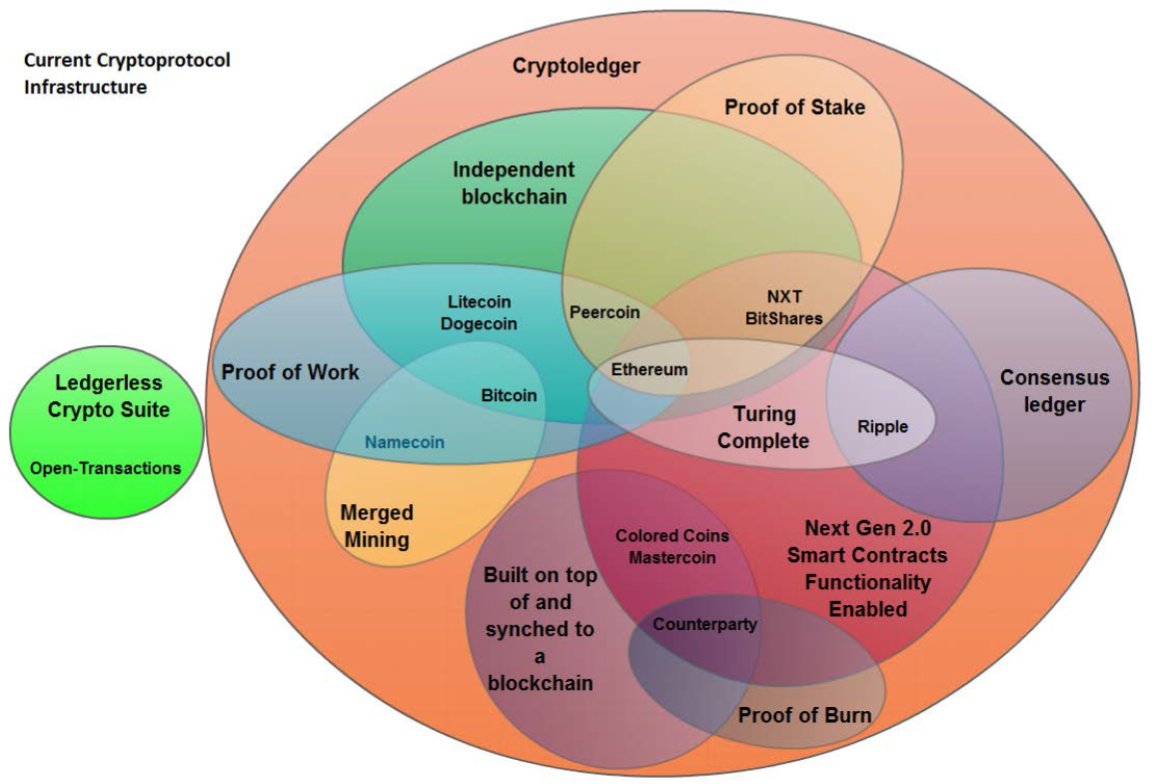
\includegraphics[width=0.8\textwidth]{./images/current_protocols}
    \caption{Классификация на 2014 год \cite{TimSwanson2014}}\label{2014protocol}
\end{figure}

Данная классификация представлена в книге Тима Суэнсона \cite{TimSwanson2014} и
являлась актуальным на 2014 год представлением классификации криптографических
алгоритмов и протоколов для распределённых реестров. Сегодня, когда появилось
множество новых алгоритмов и были изобретены уникальные типы реестров, данная
классификация утратила свою значимость и нуждается в обновлении и
актуализации. В рамках данной работы будет представлена новая классификация
алгоритмов и протоколов для распределённых реестров. Классификация сохранит
принципы построения и представления своего предшественника.

\subsubsection{Программная составляющая}
Программной составляющей настоящего проекта является приложение из двух частей:
\begin{my_enumerate}
    \item Позволяющей сгенерировать код блокчейна с использованием выбранных
          пользователем алгоритмов
    \item Является выходом первой компоненты, и по своей сути обособленным приложением --- блокчейном
\end{my_enumerate}
В дальнейшем (1) будет именоваться \textbf{компоновщик}, а (2) --- \textbf{реализация блокчейна}. 

\paragraph{Codecreator.com}
Данный ресурс \cite{CodeCreator} (на вкладке blockchain) представляет собой
сервис, предназначенный для развёртывания реестра на сервере Amazon AWS. Ресурс
позволяет развернуть реестры, основанные на Ethereum и Hyperledger. Ресурс
предназначен для крупных бизнес проектов, требующих рабочий код быстро. Имеет
бесплатную пробную версию.

\paragraph{Azure BaaS}
Данная платформа \cite{MicrosoftAzure}, Microsoft Azure Blockchain as a
Service, обеспечивает быструю, относительно недорогую, платформу для создания и
развертывания блокчейн-приложений. Azure предлагает Blockchain как сервис
(BaaS), а значит, встраивание кода блокчейна в код не предусматривается. Есть
поддержка самых популярных реестров, таких как Ethereum, Quorum, Hyperledger
Fabric, Corda.

\paragraph{Magic Code Generator}
Релиз данной платформы \cite{mcg} ещё не состоялся.  Документы, содержащиеся на
страницах описывают сервис, предназначенный для построения приложений,
взаимодействующих с сетями реестров. Например, онлайн биржу валют. Так же
сервис имеет возможность создания blockchain-based приложений.


Данный проект \emph{прямым} аналогом ни одного из приведённых приложений не
является. Это позволяет сказать, что проект уникальный в своём роде. Тем не
менее, есть сходства и различия, по которым можно привести следующее сравнение
(Табл. 1).

\begin{center}
    \begin{tabular}{ | p{4cm} | c | c | c | c | }
    \hline
    \hline
      Признак & Codecreator & Azure BaaS & MagicCodeGenerator\footnotemark & \textbf{GSL} \\ \hline
      Встраивание кода в своё приложение & Частично & Частично & --- & \textbf{Да} \\ \hline
      Моментальное развёртывание & --- & --- & --- & \textbf{Да} \\ \hline
      Вариаций алгоритмов использования & < 5 & < 10 & 0 & \textbf{24} \\ \hline
      Стоимость & $\approx$5600 руб./мес. & $\approx$3300 руб./мес. & Не известно & \textbf{0 руб. / мес.} \\ \hline
    \hline
  \end{tabular}

    \vspace{-5cm} \hfill \emph{Таблица 1. Сравнение с аналогами} \vspace{4.1cm}
\end{center}

\footnotetext{Релиз MagicCodeGenerator ещё не состоялся.}


\newpage

\subsection{Источники для изучения}
Источниками для изучения тематических материалов, отслеживания свежих обновлений информации и публикаций будут служить:

\begin{itemize}
    \item Топик ``Блокчейн'' на https://www.researchgate.net/topic/Blockchain
    \item Топик ``Криптография'' на https://www.researchgate.net/topic/Cryptocurrency
    \item Книга Great Chain of Numbers (Swanson, Tim) \cite{TimSwanson2014}
    \item Тред ``r/Blockchain'' на https://www.reddit.com/r/BlockChain/
    \item Тред ``r/CryptoCurrency'' на https://www.reddit.com/r/CryptoCurrency/
    \item Статьи на https://medium.com/
    \item Статьи на https://wikipedia.org/
\end{itemize}



\subsection{Виды распределённых реестров}\label{kinds_reestrs}
Для классификации алгоритмов и протоколов по распределённым реестрам и
их семействам, был проведён обзор используемых в настоящие дни их
представителей.\\
Для разделения реестров на группы по признакам открытости и закрытости
существует несколько подходов.
\begin{itemize}
    \item Первый --- канадский, основанный на публикации статьи
        \cite{VitalikButerin2015} создателя криптовалюты Ethereum Виталика
        Бутерина. Автор разделяет 3 типа реестров:
          \begin{enumerate}
              \item Публичный (Public), где каждый может принять участие в
                  создании блоков, которое никем не контролируются и
                  выполняется в свободном порядке;
              \item Приватный (Fully Private), где все транзакции отслеживаются
                  и контролируются централизованной сущностью;
              \item Реестры консорциума (Consortium), где только избранные узлы
                  цепи контролируют создание новых блоков.
          \end{enumerate}
     \item Второй --- британский. Определения Сэра Марка Уолпорта, главного
         научного советника Соединённого Королевства, в докладе о
         распределённых реестрах \cite{DeLeon2018}, совпадают по своей сути с определениями
         Бутерина, но отличаются названиями:
         \begin{enumerate}
                 \item Unpermissioned public;
                 \item Permissioned private;
                 \item Permissioned public.
         \end{enumerate}
     \item Третий --- \textbf{российский}. Часто, для избежания недопониманий и
         сложностей в определении, мировые эксперты используют понятия
         Публичный (Открытый) и Приватный (Закрытый) реестры. Российские
         эксперты не исключение. В своём докладе \cite{2016}, Ольга Скоробогатова,
         заместитель председателя ЦБ РФ, разделяет реестры именно таким
         образом. Данное разделение будет использоваться в настоящей работе:
         \begin{enumerate}
             \item Публичный (Открытый, Public, Open). В открытых реестрах нет
                 контролирующей стороны, как это реализовано в закрытых
                 реестрах, все транзакции происходят в свободном порядке, а для
                 подтверждения легитимности транзакции используются специальные
                 протоколы консенсуса (\ref{consensus_protocols})
             \item Приватный (Закрытый, Private, Closed). Несмотря на то, что
                 сама рассматриваемая технология является распределённой,
                 элементы централизованности присутствуют в таких вариантах,
                 как закрытые (\ref{kinds_reestrs}) реестры. Закрытым реестр
                 может являться благодаря первичному блоку (в случае
                 блокчейна), который будет использоваться. Любой узел может
                 присоединиться к приватному реестру, если он знает адрес
                 начального узла для синхронизации и идентификатор сети. Этот
                 узел может выполнять любые действия в закрытом реестре:
                 майнить, совершать транзакции, заключать контракты, и т.д.\\

                 Такие реестры зачастую используюся фирмами, банками и т.д. для
                 организации внутренних операций обмена и регистрирования.
         \end{enumerate}
\end{itemize}

\subsection{Структура реестров}
По своей внутренней структуре распределённые реестры делятся на
блокчейны (\ref{struct_block}) и направленные ациклические графы
(\ref{struct_dags}). На рисунке \ref{graph_reester} изображены виды современных
распределённых реестров.

\begin{figure}[h]
    \Tree [.DL [.DAG ] [.Blockchain ] [.Hybrids\ \&\ Others ]]
    \caption{Виды распределённых реестров}\label{graph_reester}
\end{figure}

\subsubsection{Блокчейны}\label{struct_block}
Блокчейны --- наиболее распространённые сегодня виды реестров. Набор транзакций
(операций) собирается в один блок. Проходит определенное время и этот блок
добавляется в общую цепочку. Для подтверждения транзакции существует множество
протоколов консенсуса --- стандартов, исходя из которых можно говорить, что
создание и добавление данного блока имеет место быть. Подтверждение легальности
добавления блоков в других представлениях распределённых реестров происходит с
применением других алгоритмов и протоколов, поэтому далее для протоколов
консенсуса будет использоваться слово ``блокчейн'' вместо ``реестр'' для
исключения возможности двоякой интерпретации (на самом деле, в некоторых
реализациях DAG \cite{Popov2018} может применяться протокол консенсуса
Proof-of-Work \ref{pow} для защиты от спама). Блокчейны завоевали
стратегические позиции на площадке распределённых реестров и ``прошли проверку
временем'', но появляются новые технологии, такие как DAG и другие, призванные
решить некоторые недостатки сетей блокчейн, речь о которых пойдёт позднее.

\subsubsection{Направленные ациклические графы (DAGs)}\label{struct_dags}
В DAG все новые записи добавляются в общую цепочку (корректнее --- граф)
асинхронно. История записи операций выглядит как направленный ациклический граф
(\cite{wikii}). DAG топологически отсортирован так, что каждое ребро направлено
от более раннего ребра к более позднему.

\subsubsection{Плюсы и минусы DAG}
Рассмотрим некоторые преимущества и недостатки DAG по отношению к блокчейнам.\\
Плюсы:
\begin{itemize}
    \item Масштабируемость
    \item Мгновенные транзакции
    \item Отсутствие либо чрезмерно малые (незаметные) комиссии за переводы
\end{itemize}
Эти плюсы открывают дорогу для огромного количества микротранзакций, делая
систему пригодной, для, например, интернета вещей.\\
Минусы:
\begin{itemize}
    \item Возможные в будущем проблемы с масштабируемостью
    \item Нет подтверждённой учёными информации о защите от взлома основанных на DAG систем
\end{itemize}

\subsection{Алгоритмы}
Рассмотрим некоторые криптографические алгоритмы, которые используются в описанных системах.
\subsubsection{SHA-256}
\emph{Используется в таких реестрах как: } \textbf{Bitcoin, ILCoin}\\\\
Алгоритм хэширования SHA-256, работая с данными, разбитыми на кусочки по 512
бит (64 байт), смешивает их криптографически и выдаёт 256-битный (32 байта) хэш
--- уникальную (почти: \cite{Jim2012}) сигнатуру входного текста.
\subsubsection{ECDSA}
\emph{Используется в таких реестрах как:} \textbf{Bitcoin} \\\\
Алгоритм цифровой подписи ECDSA (Elliptic Curve Digital Signature Algorithm)
--- криптографический алгоритм, используемый в целях гарантировать, что узлы
сети могут быть использованы только их законными владельцами. Использует
концепты публичного и приватного ключа. В алгоритме публичный ключ --- это
уравнение для эллиптической кривой (Рис. \ref{elliptic_curve}) и точка, лежащая
на этой кривой. Приватный ключ --- это простое число.

\begin{figure}[h]
    \centering
    \begin{tikzpicture}
        \begin{axis}[
            xmin=-2,
            xmax=4,
            ymin=-7,
            ymax=7,
            xlabel={$x$},
            ylabel={$y$},
            scale only axis,
            axis lines=middle,
            % set the minimum value to the minimum x value
            % which in this case is $-\sqrt[3]{7}$
            domain=-1.912931:3,      % <-- works for pdfLaTeX and LuaLaTeX
            % domain=-1.91293118:3,   % <-- would also work for LuaLaTeX
            samples=200,
            smooth,
            % to avoid that the "plot node" is clipped (partially)
            clip=false,
            % use same unit vectors on the axis
            axis equal image=true,
        ]
            \addplot [blue] {sqrt(x^3+7)}
                node[right] {$y^2=x^3+7$};
            \addplot [blue] {-sqrt(x^3+7)};
        \end{axis}
    \end{tikzpicture}
    \caption{Эллиптическая кривая}\label{elliptic_curve}
\end{figure}

\newpage
\subsection{Прочие алгоритмы}
Помимо стандартных криптографических алгоритмов шифрования, генерации
электронной подписи и случайных чисел, в распределённых реестрах повсеместно
используются алгоритмы, обеспечивающие сокрытие персональных данных и адресов
отправителей и получателей, алгоритмы по защите и обфусцированию данных,
отправляемых по небезопасным каналам связи.
\subsubsection{Ring Signatures}
\emph{Используется в таких реестрах как: } \textbf{Monero, Particl, Bytecoin} \\\\
Представлен впервые в Декабре 2012 \cite{VanSaberhagen2012} Cryptonote. Вторая версия документа
Cryptonote v2 --- Октябрь 2013 \cite{VanSaberhagen2013}.
Такая криптовалюта как Monero использует технологию кольцевой
подписи для защиты конфиденциальности пользователя при проведении транзакций.
Кольцевые подписи скрывают информацию об отправителе, заставляя отправителя
подписывать транзакцию с помощью подписи, которая может принадлежать нескольким
пользователям. Это делает транзакцию неотслеживаемой.\\
Интересно рассмотреть вариацию данного алгоритма RingCT, которая будет
рассмотрена далее (\ref{ringct})
\subsubsection{Stealth Addressess}
\emph{Используется в таких реестрах как: } \textbf{Monero, Particl, Bytecoin} \\\\
Представлены в том же документе. Stealth addresses позволяют получателю
предоставлять для получения один адрес, который генерирует другой публичный
адрес для средств, которые будут получены каждый раз при отправке на него. Это
делает транзакцию также, неотслеживаемой.\\

Поскольку алгоритмы определены в одной работе и имеют схожие цели, можно,
объединив их, назвать основные плюсы и минусы:\\
\textbf{Плюсы}
\begin{itemize}
    \item Обеспечивает конфиденциальность отправителя и получателя
    \item Конфиденциальность может гарантироваться по умолчанию
    \item Проверенная технология
    \item Не требует каких-либо третьих сторон
\end{itemize}
\textbf{Минусы}
\begin{itemize}
    \item Конфиденциальность не очень эффективна, имея недостаточный объем
          хранилища
    \item Не скрывает информацию о самой транзакции (если алгоритм
          используется сам по себе, не объединяясь с другими)
\end{itemize}

\subsubsection{Coinjoin, coinshuffle}
\emph{Используется в таких реестрах как: } \textbf{ Dash } \\\\
Разработчик Биткоина Грегори Максвелл предложил набор решений для обеспечения
конфиденциальности в распределённых реестрах и криптовалютах, первым из которых
являлся CoinJoin. \cite{Maurera}. CoinJoin (иногда называемый CoinSwap)
позволяет нескольким пользователям объединять свои транзакции в одну
транзакцию, получая входы от нескольких пользователей, а затем отправляя свои
выходы нескольким пользователям, независимо от того, от кого в группе пришли
входы. Таким образом, получатель получит назначенную сумму, но будет
невозможным отследить транзакцию вплоть до отправителя.\\
\textbf{Плюсы}
\begin{itemize}
    \item Обеспечивает конфиденциальность отправителя и получателя
    \item Простота реализации на любой криптовалюте
    \item Легковесная реализация в коде
    \item Проверенная технология
\end{itemize}
\textbf{Минусы}
\begin{itemize}
    \item Суммы смешанных транзакций могут быть высчитаны
\end{itemize}

\subsubsection{Sigma Protocol}
\emph{Используется в таких реестрах как: } \textbf{Zcoin} \\\\
Sigma Protocol --- активно исследуется командой Zcoin с 2018 года для замены
протокола Zerocoin zk-Snarks (zero knowledge succinct non-interactive arguments of
knowledge) для того, чтобы не требовалась доверенная
преднастройка. \cite{Groth2015}. Существует возможная замена zk-Snarks,
называемая zk-Starks, другая форма доказательства нулевого знания, которая
может сделать доверенную преднастройку ненужной для монет с нулевым знанием.

\subsubsection{Zerocash}
\emph{Используется в таких реестрах как: } \textbf{ Zcash, Horizen, Komodo, Zclassic, Bitcoin Private } \\\\
В мае 2014 года был создан нынешний преемник протокола Zerocoin, Zerocash. Он
улучшил концепцию Zerocoin, воспользовавшись уже известным zk-Snarks. В отличие
от Zerocoin, который скрывал происхождение оригинальных монет и историю
платежей, Zerocash был быстрее, с меньшими размерами транзакций и скрывает
информацию о транзакции отправителя, получателя и суммы транзакций.
Zcash-первая криптовалюта, реализовавшая протокол Zerocash в 2016 году.
\cite{ZerocoinElectricCoinCompany2016}

\subsubsection{CT, RingCT}\label{ringct}
\emph{Используется в таких реестрах как: } \textbf{Monero, Particl} \\\\
Confidential Transactions были представлены обществу в 2015 году \cite{Maxwell}
Было предложено скрыть сумму транзакции и тип передаваемых данных (например,
депозиты, валюты, акции), чтобы только отправитель и получатель знали о сумме
(до тех пор, пока они не решат сделать сумму общедоступной). В алгоритме
используется гомоморфное шифрование для шифрования входов и выходов.\\

Затем появились Ring Confidential Transactions \cite{Noether2016}.  RingCT
сочетает использование кольцевых подписей для сокрытия информации об
отправителе с использованием конфиденциальных транзакций (которые также
используют кольцевые подписи) для сокрытия сумм. В работе описан новый тип
кольцевой подписи --- A Multi-layered Linkable Spontaneous Anonymous Group,
многослойная связанная спонтанная анонимная групповая подпись, которая
``позволяет скрывать суммы, происхождение и назначение транзакций, с разумной
эффективностью и качественной проверкой, с возможностью не-доверительной
генерации монет''.

\subsubsection{MimbleWimble}
\emph{Используется в таких реестрах как: } \textbf{Grin} \\\\
Mimblewimble \cite{Poelstra2016} использует концепцию Confidential Transactions
для скрытия сумм, а для доказательства права на собственность, смотрит на
закрытые ключи и информацию о транзакциях, а не на адреса, также, связывает
транзакции вместе, а не рассматривает их отдельно на блокчейне. Grin --- это
криптовалюта, находится в состоянии разработки и применяет Mimblewimble.

\subsubsection{Zexe}
В Октябре 2018 Zexe был представлен новый криптографичекий концепт ---
``децентрализованные частные вычисления'' (decentralized private computation)
\cite{Bowe2019}. Он позволяет пользователям распределённых реестров ``выполнять
автономно вычисления у себя на машинах, результатами которых будут настоящие
транзакции'', а также сохраняет суммы транзакций скрытыми и позволяет проверять
транзакции в любое время независимо от вычислений, выполняемых в интернете.

\subsection{Протоколы консенсуса}\label{consensus_protocols}
Протокол консенсуса --- стандарт, описывающий правила создания блоков в
открытых распределённых реестрах. В работе рассмотрены все протоколы
консенсуса, используемые в распространённых на сегодняшний день распределённых
реестрах.
\subsubsection{Proof of Work (PoW)}\label{pow}
\emph{Используется в таких реестрах как: } \textbf{Bitcoin, Litecoin, Dogecoin} \\\\
Впервые концепция Proof of Work была описана в 1993 году в работе ``Pricing via
Processing, Or, Combatting Junk Mail, Advances in Cryptology''
\cite{Dwork2007}.

Идея авторов заключалась в следующем: чтобы получить доступ к общему ресурсу,
пользователь должен вычислить некоторую достаточно сложную функцию, и так
защитить ресурс от злоупотребления.  В 1997 году Адам Бэк запустил проект
Hashcash, посвященный той же защите от спама. Задача формулировалась следующим
образом: «Найти такое значение x, что хеш SHA(x) содержал бы N старших нулевых
бит».

Алгоритм PoW используется в открытых реестрах
для создания новых блоков. Алгоритм хорошо проявляет себя для доказательства
легитимности транзакции, выполняя которое, майнеры вознаграждаются процентом,
соответствующим вычислительной сложности всей сети. Зарекомендовавшее себя
средство, оно не является выгодным с точки зрения расхода природных ресурсов,
поскольку объём энергозатрат для выполнения вычислений, необходимых на
добавление одного блока, сопоставим с объемом энергии, потребляемым двумя
средними американскими домами: `` Bitcoin transaction uses roughly enough
electricity to power 1.57 American households for a day.'' --- \cite{amhouses}

\subsubsection{Proof of Stake (PoS)}
\emph{Используется в таких реестрах как: } \textbf{Ethereum} \\\\
Алгоритм доказательства доли владения --- основной конкурент предыдущего
алгоритма. Вероятность формирования участником очередного блока в реестре
пропорциональна доле, которую составляют принадлежащие этому участнику
расчётные единицы данного реестра (напр., кол-во единиц криптовалюты) от их
общего количества. Поскольку для принятия решения о том, кто будет являться
создателем нового блока, нет необходимости в большом объёме вычислений, как в
PoW, зачастую является выбором, когда экологический фактор поставлен на одно из
главных мест.

\subsubsection{Delegated Proof-of-Stake (DPoS)}
\emph{Используется в таких реестрах как: } \textbf{Oxycoin, Lisk, Ark} \\\\
Delegated PoS применяет PoS с расширенным функционалом. Поэтому остается
быстрым (и даже ещё быстрее), не требует больших вычислительных мощностей по
сравнению с алгоритмом Proof of Work (PoW). Суть DPoS состоит в том, что узлы
сети методом голосования выбирают узел, который будет генерировать блоки. В
этом случае работает правило: чем большим количеством монет обладает узлы, тем
больший вес имеет ее голос. Правила начисления вознаграждения также
определяются также участниками сети. В некоторых сообществах вознаграждение
начисляется не только узлы, которой делегировали право генерировать блоки, но и
остальным участникам. Первая криптовалюта, в которой был применен алгоритм DPoS
--- Bitshares. Также он применяется в следующих проектах: EOS, Steemit.

\subsubsection{Proof-of-Authority (PoA)}
\emph{Используется в таких реестрах как: } \textbf{POA Network} \\\\
Алгоритм доказательства полномочий --- это ещё один алгоритм консенсуса, в
котором транзакции проверяются специальными учетными записями (валидаторами)
системы. То есть майнить могут только валидаторы. Как пример использования
можно привести систему Kovan Testnet \cite{Etherium2018}.

\subsubsection{Byzantine Fault Tolerance (BFT)}
\emph{Используется в таких реестрах как: } \textbf{NEO (dBFT)} \\\\
Лэсли Лэмпорт в 1982 году \cite{Lamport2002} со своими соавторами представили
общественности задачку о Византийских генералах, позже использованную для
создания алгоритма консенсуса BFT.

В BFT, как и в PoA существуют валидаторы, и только им позволено совершать
быстрые транзакции, управлять каждым состоянием сети и обмениваться сообщениями
друг с другом, чтобы получить правильную запись транзакции и обеспечить
честность. Данный алгоритм реализуется компанией Ripple, где валидаторы
выбираются предварительно. Любой может быть валидатором --- доверие
устанавливается сообществом. В отличие от блокчейнов, основанных на PoW,
блокчейны BFT не подвергаются нападению, если только сами пользователи сети не
координируют атаку. BFT считается выгодным алгоритмом, поскольку он
масштабируем и охватывает транзакции с низкой стоимостью, но, как и DPoS,
внедряет компонент централизации.

\subsection{Выводы по главе}
В данной главе были рассмотрены основные и наиболее распространённые алгоритмы
и протоколы в распределённых реестрах сегодняшнего дня. Поскольку в расчёт
брались только популярные, этого должно хватить для понимания общей картины
текущего криптопротокола, но работа нацелена на глубокое изучение. На рис.
\ref{2014protocol} \cite{TimSwanson2014} приведена структура используемых
алгоритмов и протоколов в распределённых реестрах на 2014 год. На сегодняшней
день многое поменялось и добавились новые алгоритмы и протоколы, появились
новые распределённые реестры, не основанные на блокчейне. В качестве
результата проведённого изучения алгоритмов и протоколов в данной работе, на
рис.\ref{myprotocol} приведена классификация обновлённая, на Q2 2019 года. На
ней очевидны изменения в количественную сторону.

\newpage

\begin{figure}[h!]
    \centering
    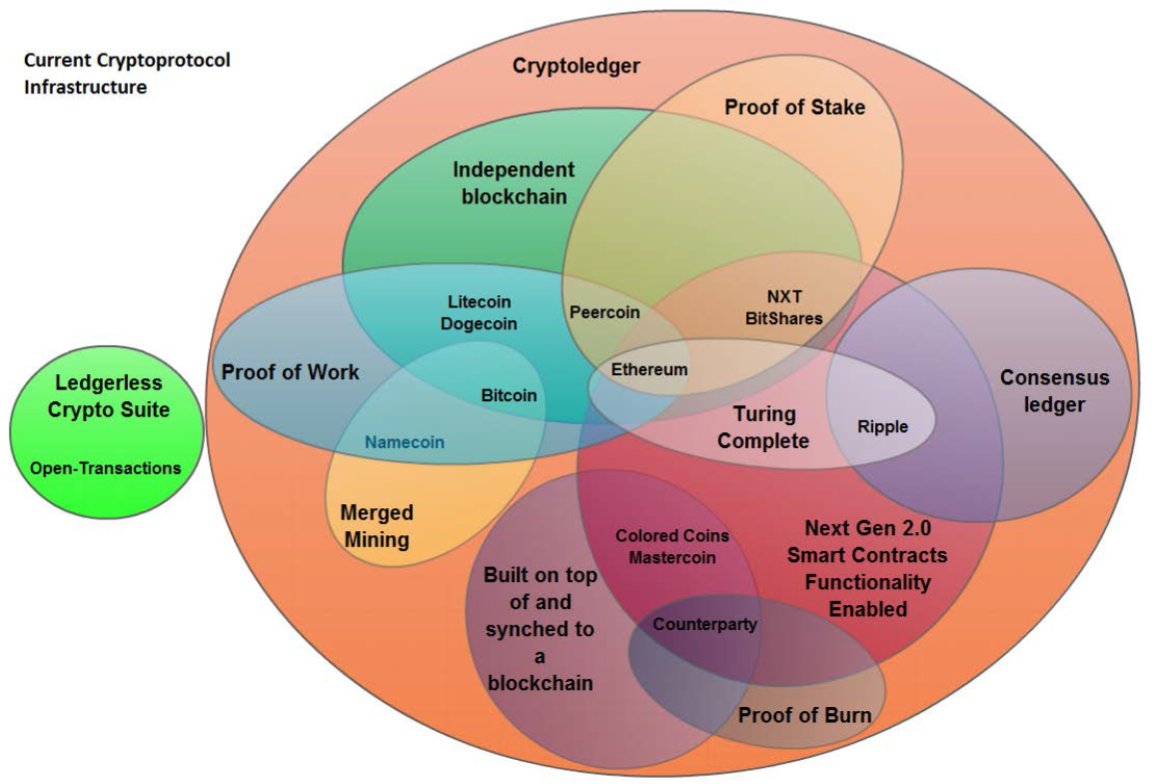
\includegraphics[width=0.78\textwidth]{./images/current_protocols}
    \caption{Классификация на 2014 год \cite{TimSwanson2014}}\label{2014protocol}
\end{figure}


\begin{figure}[h!]
    \centering
    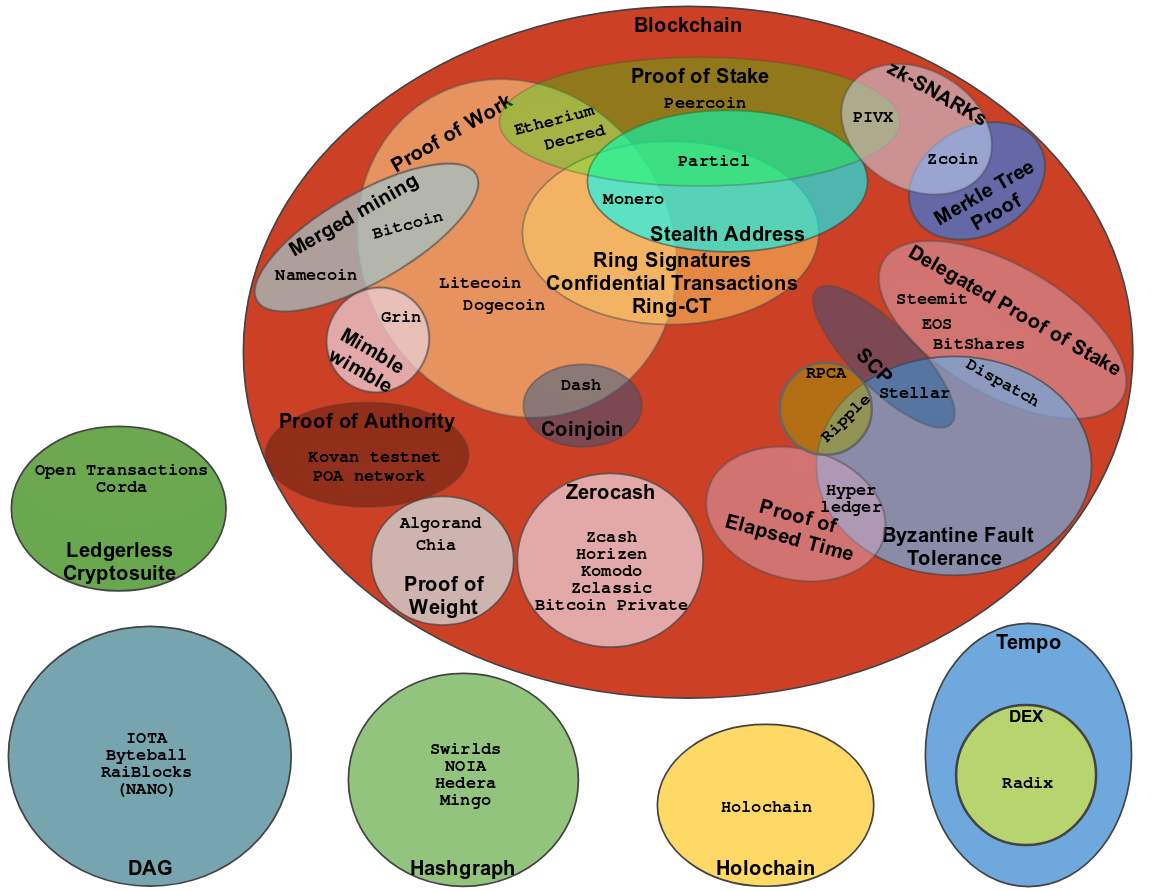
\includegraphics[width=0.9\textwidth]{./images/myprotocol}
    \caption{Классификация на 2019 год}\label{myprotocol}
\end{figure}


\newpage
\section{Глава 2. Проектирование сервиса: архитектура, процессы}
В данной главе рассматриваются особенности реализации сервиса для
автоматизации программирования с использованием технологии блокчейн на основе
различных алгоритмов. В начале приведены архитектурные составляющие проекта
\textbf{с обоснованием использования} средств реализации приведённой
архитектуры, далее --- функциональные, а в заключении собраны выводы по главе.

\subsection{Архитектурные особенности}
\subsubsection{Общая структура проектного решения}
Глобально проект состоит из двух компонент. Первая отвечает за интерактивное
взаимодействие с пользователем и генерацию кода второй компоненты с
использованием указанных пользователем алгоритмов (далее --- компоновщик).
Вторая --- это имплементация блокчейна (далее --- реализация блокчейна).
Проект содержит код для кошелька ({\small wallet.py}) и майнера ({\small
miner.py}) с определённой функциональностью. Код второго проекта структурирован
для удовлетворения нужд использования указанных пользователем методов. Методы и
классы генерируются at-runtime первого приложения.

\paragraph{Язык программирования}
Использованный язык программирования --- \textbf{Python} верисии
\underline{3.6.5}.\\
\emph{Рассматриваемые аналоги}: C, Java\\\\
Выбран вследствие своей универсальности применения
относительно (а) алгоритмов, (б) платформы для запуска; а также простоты
реализации побочных, вспомогательных компонент, посредственно относящихся к
данному проекту. Реализация их на других языках была бы необходимостью --- и, в
следствии их посредственного отношения к проекту, необоснованной тратой
временного ресурса.\\
\emph{Реализации алгоритмов \textbf{keccak-256 \emph{ и } keccak-512} были
переписаны с Python2 на Python3.6.5 для совместимости с данной программой}.

\paragraph{Тип приложения}
Приложение является консольной утилитой, которая может быть установлена в
систему семейства \underline{GNU/Linux} при помощи программы
\textbf{python3-pip}.\\
\emph{Рассматриваемые аналоги}: Приложение с графическим интерфейсом,
приложение в веб-интерфейсом\\\\
Отсутствие графического интерфейса обосновано отсутствием
необходимости произведения манипуляций при помощи мыши, и отсутствием
необходимости отображения графических изображений и другой информации.
Интерактивный диалог производится посредством вывода в стандартный выход
(\emph{stdout}) консоли текста с опциями; а выбор пользователя регистрируется
посредством считывания стандартного ввода (\emph{stdin}).

\paragraph{Протокол обмена данными между компонентами}
Выбранной опцией является передача \textbf{json} файлов посредством \textbf{http} протокола.\\
\emph{Рассматриваемые аналоги}: \textbf{grpc} \cite{grpc}, \textbf{zmq} \cite{zmq}\\\\
Обеспечивается использованием модуля \emph{Flask} \cite{flask} и \emph{json}. В сравнении
с \emph{grpc} и \textit{zmq} протоколами, \emph{http}
представлялся наиболее подходящим вследствие своей популярности и удобства
подключения и использования совместно с языком Python.

\paragraph{Хранилище}\label{hraaan}
В качестве хранилища было реализовано \textbf{key-value} (ключ-значение) хранилище.\\
\emph{Рассматриваемые аналоги}: \textbf{etcd} \cite{etcd}, \textbf{sqlite} \cite{sqlite}\\\\
Подключение сторонней библиотеки или базы данных сильно увеличило бы вес
приложения в целом, а также добавило бы ещё несколько зависимостей. Вследствие
этого было решено придумать импровизированное key-value хранилище на основе
структуры данных словарь (dictionary).
Реализация и функциональность описана в настоящем техническом задании
(Приложение 1).
% (Приложение \ref{tz}).

\paragraph{Автообновление}
Задачей автообновления занимается UNIX утилита \textbf{cron}.\\
\emph{Рассматриваемые аналоги}: Импровизированный планировщик событий\\\\
В связи с существованием качественного и надёжного решения в лице
\textbf{cron}'a, было решено использовать его. Настроен на сервере. Подробнее
--- в п. \ref{autoobnova}

\paragraph{Continuous integration}
В качестве средства CI был выбран \textbf{Shippable} \cite{shippable}.\\
\emph{Рассматриваемые аналоги}: \textbf{TravisCI} \cite{travisci}, \textbf{CircleCI} \cite{circleci}\\\\
Данное средство распространяется с возможностью использовать бесплатную версию
программы, поэтому выбор пал на неё. \emph{Необходимость} в сервисе CI
выражается в том, чтобы данное приложение генерировало рабочие стабильные коды
даже после обновления используемых реализаций алгоритмов, что не зависит от
разработчика.

\paragraph{Конфигурация}
Конфигурационный файл программы написан на языке \textbf{YAML} \cite{yaml}.\\
\emph{Рассматриваемые аналоги}: \textbf{JSON}, \textbf{Plain text}\\\\
Выбран \emph{YAML} по причине хорошей поддерживаемости в Python и своей эстетической
непритязательности по сравнению с аналогами.




\subsubsection{Архитектура компоновщика}
Компоновщик --- часть проекта, автоматизирующая процесс программирования и
позволяющяя тем самым создавать готовые решения. Решением может быть рабочий
код блокчейна с использованием 24 вариаций алгоритмов.

\subsubsection{Порядок работы компоновщика}
Программно компоновщик был назван {\small gsl}. Основная команда с которой
придётся иметь дело --- init. Пример:\\

\begin{center}
\begin{Verbatim}[frame=single]
gsl --init --name myledger --path ~/tmp/gsl
\end{Verbatim}
\end{center}

\begin{figure}[h]
    \centering
    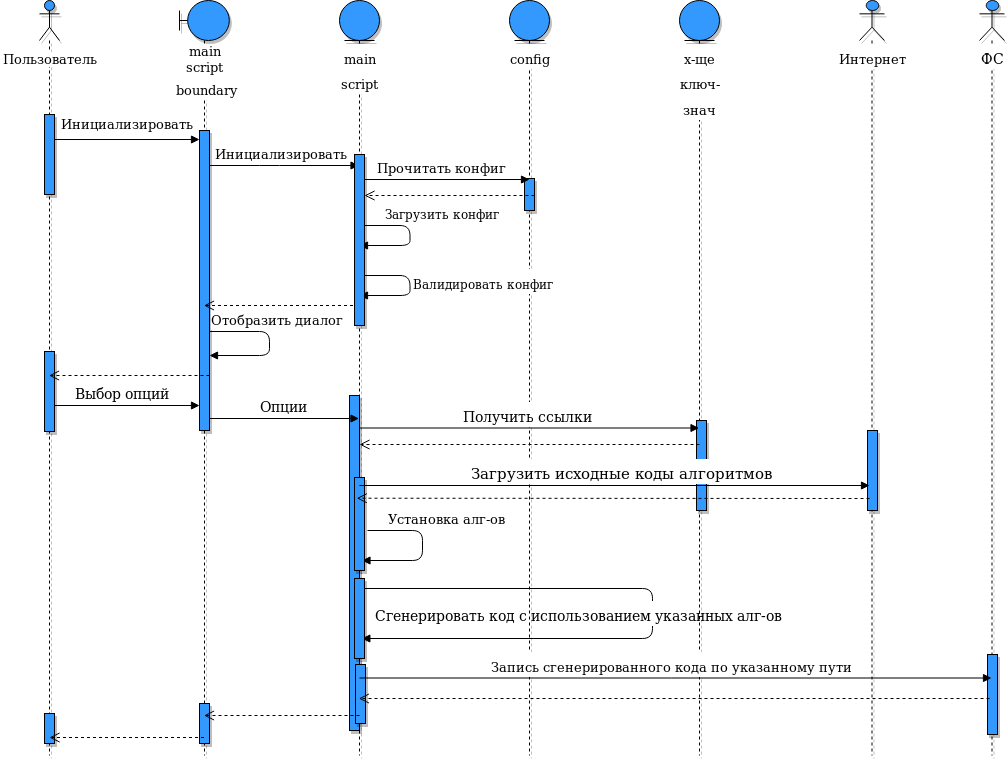
\includegraphics[width=\textwidth]{images/sequence}
    \caption{Sequence диаграмма последовательности работы первой компоненты --- компоновщика}\label{sequence}
\end{figure}

По вызову этой команды происходят процессы, обозначенные на диаграмме
последовательностей (Рис. \ref{sequence}). Зачитывается, загружается в
программу и валидируется конфигурационный файл программы.

\newpage

Затем начинается диалог с пользователем (Рис. \ref{dialog}).
\begin{figure}[h]
    \centering
    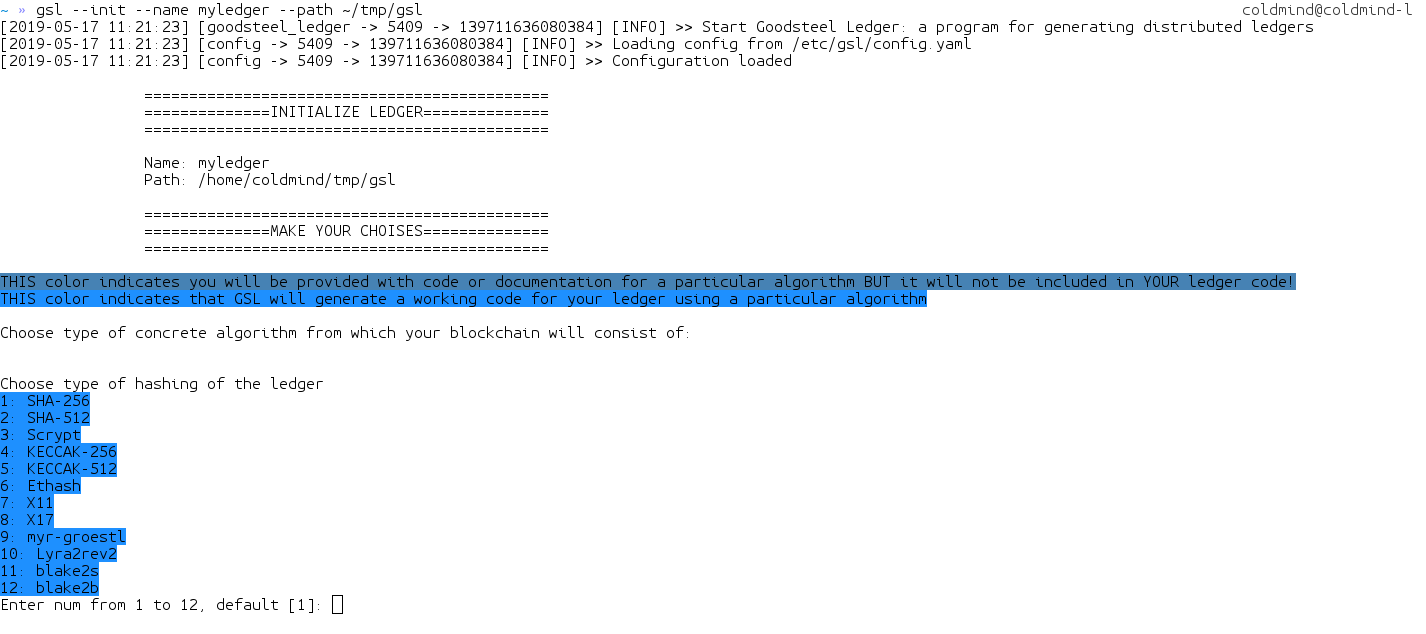
\includegraphics[width=\textwidth]{images/dialog_start}
    \caption{Начало диалога выбора алгоритмов}\label{dialog}
\end{figure}

В этом диалоге пользователь выбирает какие алгоритмы хэширования и цифровой
подписи будут использованы в его будущей реализации блокчейна. После этого,
пользователю предоставляется выбор других интересных параметров блокчейна, по
которым ему будут предложены справочные ссылки для изучения (Рис. \ref{sprav}).
После выбора происходит установка данных библиотек и генерация кода реализации
блокчейна по указанному пути (Рис. \ref{ll}).

\begin{figure}[h]
    \centering
    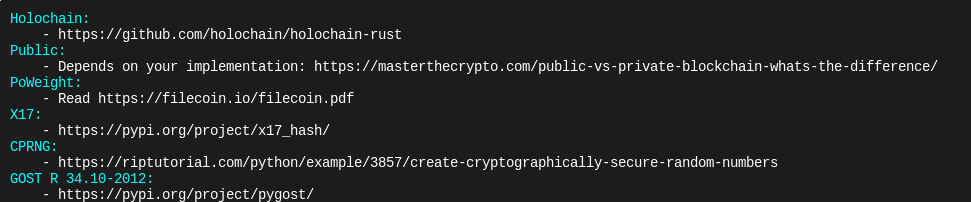
\includegraphics[width=\textwidth]{images/spravochno}
    \caption{Справочная информация по выбранным параметрам}\label{sprav}
\end{figure}

\subsubsection{Архитектура реализации блокчейна}
\begin{figure}[h]
    \centering
    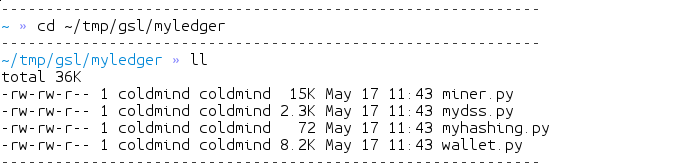
\includegraphics[width=0.8\textwidth]{images/ledger_ll}
    \caption{Директория со сгенерированным кодом реализации блокчейна}\label{ll}
\end{figure}

Код реализации блокчейна запускается интерпретатором языка Python 3.6.5.
Скрипты {\small miner.py} и {\small wallet.py} запускаются без аргументов
командной строки. Запустив {\small miner.py} (Рис. \ref{miner_run}), можно запускать {\small
wallet.py} (Рис. \ref{wallet_run}), в котором есть возможности:
\begin{enumerate}
    \item Сгенерировать кошелёк: пару публичный-приватный ключи и записать их в файл
    \item Отправить с одного кошелька на другой N условных едениц
    \item Провалидировать транзакции
\end{enumerate}

\begin{figure}[h]
    \centering
    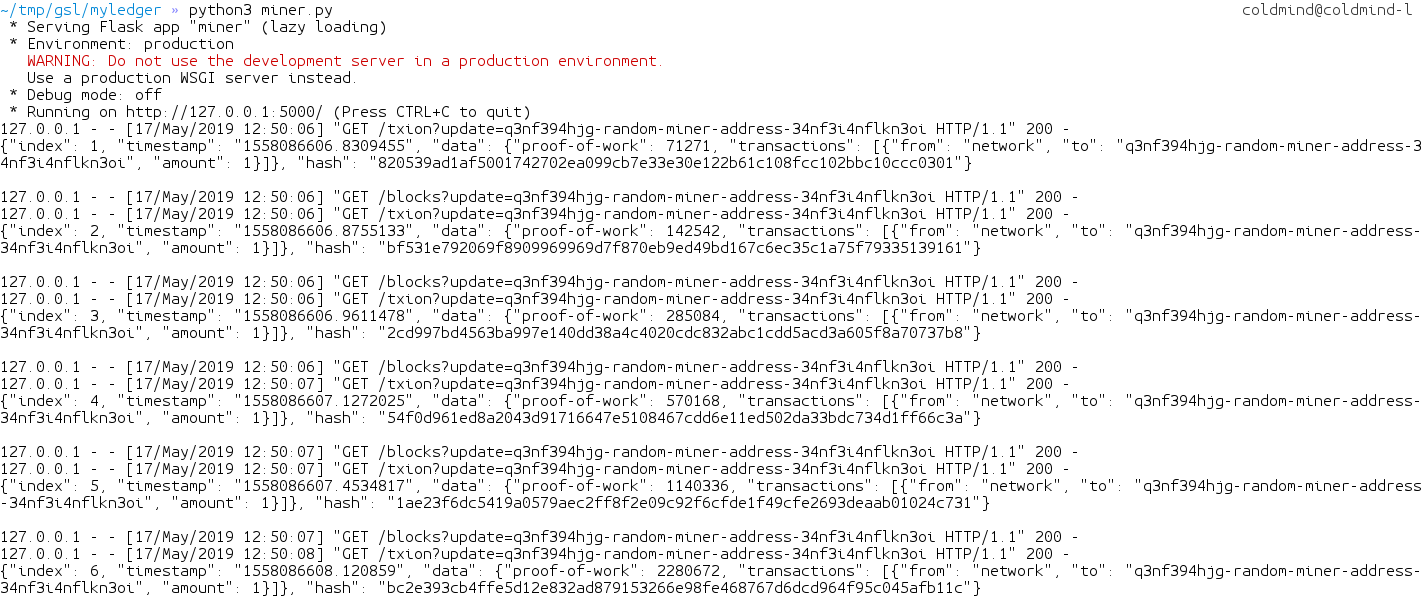
\includegraphics[width=\textwidth]{images/miner_run}
    \caption{Лог запуска майнера}\label{miner_run}
\end{figure}

\begin{figure}[h]
    \centering
    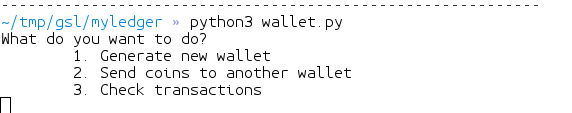
\includegraphics[width=0.8\textwidth]{images/wallet_run}
    \caption{Возможности кошелька}\label{wallet_run}
\end{figure}

Генерация пары ключей, а так же хэширование записей происходит посредством
использования выбранных ранее пользователем алгоритмов.

\newpage
\subsubsection{Работа с данными}\label{dannie_sheme}
Исходный код алгоритмов хранится в директории {\small src/altorithms/hashing} и
{\small src/altorithms/digital\_signature}. Он собирается полным проходом в
сеть по ссылкам, расположенными в импровизированном key-value хранилище
(описано в п. \ref{shron}, а так же в настоящем техническом задании ---
Приложение \ref{tz}). Данная процедура происходит при автообновлении алгоритмов
на сервере каждый день в 21:00 (Рис. \ref{update}). После процедуры
автообновления, пользователи могут по желанию обновить свою версию программы и
использовать более свежий код.

\begin{figure}[h]
    \centering
    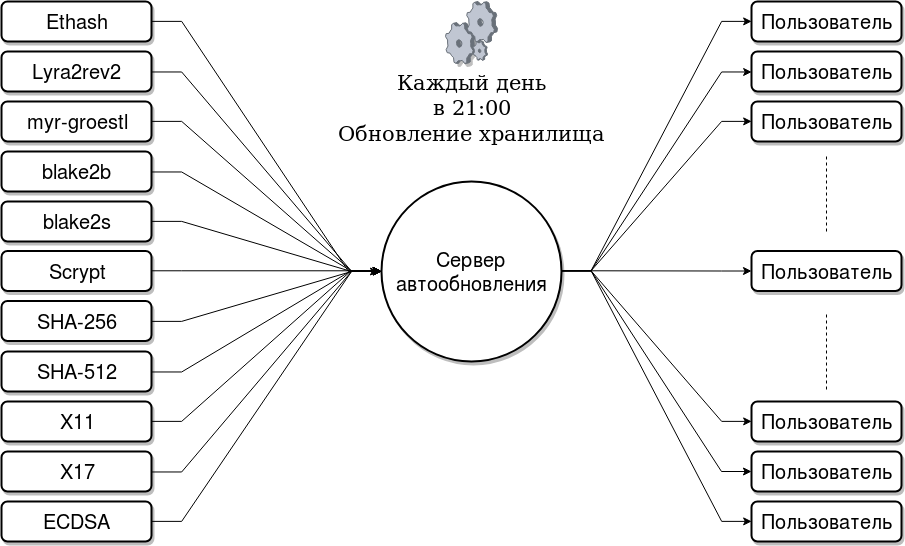
\includegraphics[width=\textwidth]{images/server}
    \caption{Процесс работы сервера автообновления}\label{update}
\end{figure}

\subsection{Функциональные особенности}


\newpage
\section{Глава 3. Программная реализация}
\subsection{Функциональные требования}
К функциональным требованиям приложения компоновщик относятся:

\begin{my_enumerate}
    \item Возможность вывода на консоль вариантов выбора по категориям:
        \begin{my_enumerate}
                \item Отображение возможных структур реестра
                \item Отображение возможных типов открытости реестра
                \item Отображение возможных алгоритмов консенсуса
                \item Отображение возможных алгоритмов хэширования
                \item Отображение возможных алгоритмов генерации случайных чисел
                \item Отображение возможных алгоритмов цифровой подписи
        \end{my_enumerate}
    \item Генерирование значений для выбора ``по умолчанию''
    \item Возможность записать выбора пользователя
    % \item Возможность поиска в хранилище ссылок для конкретных алгоритмов
    % \item Возможность загрузки из общедоступных источников исходных кодов алгоритмов
    \item Возможность установки загруженных алгоритмов на ФС машины без исключительных root прав
    \item Возможность генерировать код по указанной директории
    \item Возможность замера времени работы выбранных алгоритмов
    \item Возможность просмотра справочной информации по остальным параметрам реестра
    \item Вывод информации в цвете, обозначающий степень поддержки программой алгоритма
\end{my_enumerate}


К функциональным требованиям приложения реализация блокчейна ({\small wallet.py})относятся:
\begin{enumerate}
    \item Возможность генерации ``адреса кошелька'' --- пары приватный + публичный ключ
    \item Использование в качестве алгоритма цифровой подписи выбранный пользователем
    \item Использование в качестве алгоритма хэширования выбранный пользователем
    \item Возможность записи данных ``адреса кошелька'' на ФС машины
    \item Возможность отправки от одного пользователя другому условное
          количество условной криптовалюты
    \item Возможность получения всей цепочки транзакций, которые были проведены
          за текущую сессию путём вызова API функции майнера
\end{enumerate}

К функциональным требованиям приложения реализация блокчейна ({\small miner.py})относятся:
\begin{enumerate}
    \item Возможность принимать json сообщения по http протоколу
    \item Использование в качестве алгоритма цифровой подписи выбранный пользователем
    \item Использование в качестве алгоритма хэширования выбранный пользователем
    \item Возможность выполнения proof-of-work алгоритма
    \item Возможность добавления блока в цепочку
\end{enumerate}


\subsection{Описание реализации процесса генерации кода компоновщиком}
Процесс состоит из нескольких частей:
\begin{enumerate}
    \item Сбор опций пользователя при помощи интерактивного диалога
    \item Поиск опций в хранилище
    \item По путям из хранилища программа осуществляет поход в интернет и
          загрузку кодов алгоритмов
    \item Загруженные алгоритмы записываются на ФС машины
    \item Загруженные алгоритмы устанавливаются в систему
    \item На ФС записываются функции, обеспечивающие совместимость выбранных
          пользователем алгоритмов и реализации блокчейна
    \item На ФС записывается реализация блокчейна
\end{enumerate}

Процессы будут описываться по порядку, начиная со сбора опций.

\subsubsection{Сбор опций пользователя}

Начинается с отображения приветственного и инструкционного сообщения (Рис. \ref{dg_st})

\begin{figure}[h]
    \centering
    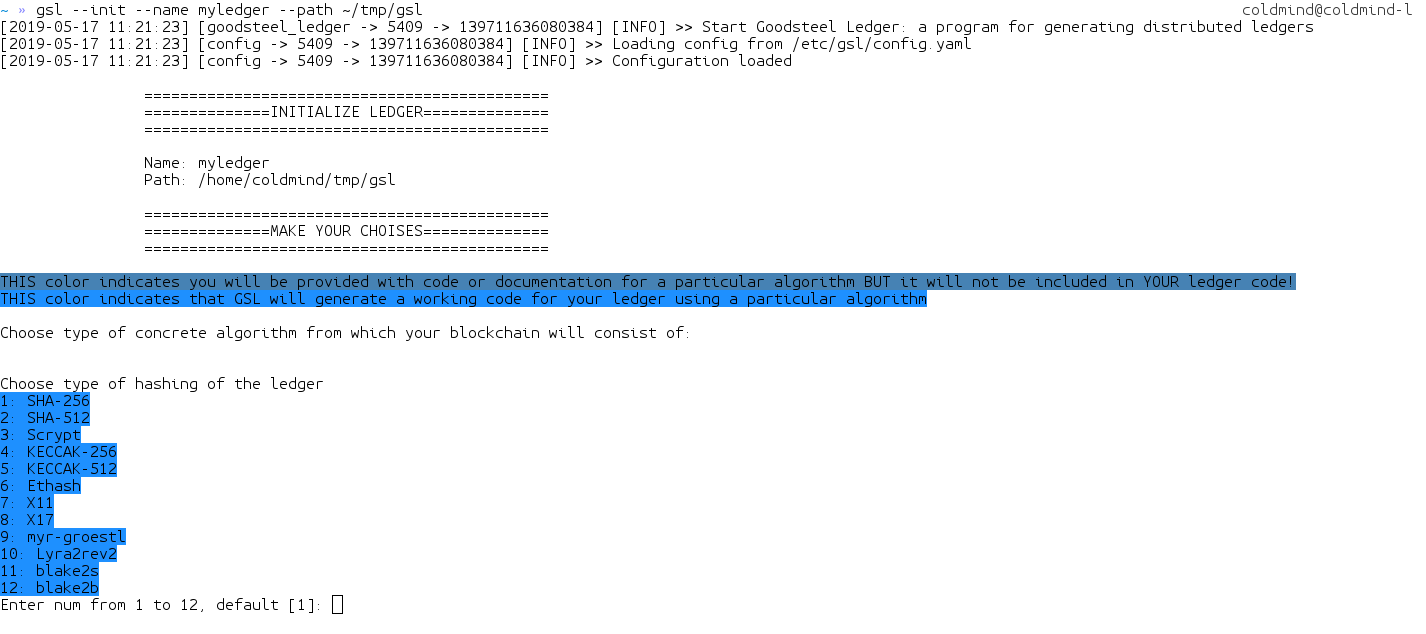
\includegraphics[width=\textwidth]{images/dialog_start}
    \caption{Начало работы компоновщика: приветственное окно и первый набор алгоритмов}\label{dg_st}
\end{figure}

В листинге \ref{print_opts} описан процесс сбора опций пользователя. Из
хранилища берётся список всех возможных опций, и согласно порядку типов
алгоритмов, распечатываются в пронумерованном виде соответствующие опции.
Пользователь затем вводит номер, размах значений которого соответствует опциям
алгоритмов данного типа. Предусмотрено значение ``по умолчанию'' для каждой из
опций --- первое значение. Вывод алгоритмов раскрашивается --- из
реализованного в рамках данной работы \textbf{utils} были импортированы функции
и константы для форматирования вывода. В случае ошибки в стандартный выход
логгера выводится её сообщение.
\begin{center}
\begin{lstlisting}
    for k, v in OPTIONS.items():
        print(f'\nChoose type of {k} of the ledger')
        if isinstance(v, list):
            for num, opt in enumerate(v):
                if 'hash' in k or 'digital' in k:
                    if opt in TOINSTALL:
                        prefix = ASCIIColors.BACK_BLUE
                    else:
                        prefix = ASCIIColors.BACK_LIGHT_BLUE
                else:
                    prefix = ASCIIColors.ENDS
                print(f'{prefix}{num+1}: {opt}{ASCIIColors.ENDS}', end='\n')
            try:
                n = input(f'Enter num from 1 to {len(v)}, default [1]: ')
                n = 0 if n == '' else int(n) - 1
                if n < 0 or n >= len(v):
                    raise ChooseError
                self.ledger_config[k] = n
            except Exception as e:
                __logger__.exception(str(e))
                return
        else:
            print(v)
\end{lstlisting}\label{print_opts}
    Листинг \ref{print_opts}: Процесс выбора опций пользователем
\end{center}

\subsubsection{Поиск алгоритмов}
На данный момент выбранные пользователем опции были получены, и записаны в переменную \textbf{options}.
Поиском алгоритмов в хранилище, интернете и их установкой на ФС машины занимается класс \textbf{ProlificWriter}.

Процесс поиска ссылок для алгоритмов в хранилище происходит путём поиска
соответствий переданных классу опций с полем хранилища \emph{TOINSTALL}. Запись
на ФС установленных алгоритмов происходит в методе \textbf{write}. Сначала
пишутся алгоритмы хэширования и электронной подписи, а затем --- код реализации
блокчейна.

\begin{center}
\begin{lstlisting}
    def write(self):
        # WRITE ALGORITHMS ITSELF
        #
        self._write_hashing_()
        self._write_digital_signature_()

        self._write_(wallet)
        self._write_(miner)


    def _write_(self, script_to_write):
        name = f'{script_to_write.__name__.split(".")[-1]}.py'
        src_code = getsource(script_to_write)
        with open(os.path.join(self.path, name), 'w') as __fd__:
            __fd__.write(src_code)
        if self.timed:
            os.system('sed -ir "0,/def _timed/{s/_timed = .*/_timed = True/}" ' + os.path.join(self.path, name))
        if self.profd:
            os.system('sed -ir "0,/def _profd/{s/_profd = .*/_profd = True/}" ' + os.path.join(self.path, name))


    def _write_hashing_(self):
        # INSTALLING PROCEDURE
        src_path = self._get_src_path_()
        path = os.path.join(src_path, get('TOINSTALL', self.opts['hashing']))
        self._install_(path)

        # WRITING PROCEDURE
        name = 'myhashing.py'
        type_ = self.opts['hashing']
        path = os.path.join(src_path, get('INTERFACES', type_), name)
        if not os.path.exists(self.path):
            os.makedirs(self.path)
        copyfile(path, os.path.join(self.path, name))

    def _write_digital_signature_(self):
        # INSTALLING PROCEDURE
        src_path = self._get_src_path_()
        path = os.path.join(src_path, get('TOINSTALL', self.opts['digital signature']))
        self._install_(path)

        # WRITING PROCEDURE
        name = 'mydss.py'
        type_ = self.opts['digital signature']
        path = os.path.join(src_path, get('INTERFACES', type_), name)
        copyfile(path, os.path.join(self.path, name))
\end{lstlisting}\label{write}
    Листинг \ref{write}: Процесс поиска алгоритмов и записи на ФС машины
\end{center}

\subsubsection{Установка}
Установка алгоритмов, упомянутая до этого в листинге \ref{write}, происходит
посредством запуска метода \_install\_, а при неудачной попытки ---
\_pip\_install\_.

\begin{center}
\begin{lstlisting}
    def _install_(self, path):
        """
        Installs with `python setup.py install`
        """
        os.chdir(path)
        subprocess.call([sys.executable, f'{path}/setup.py', 'install'])


    def _pip_install_(self, package):
        subprocess.call([sys.executable, '-m', 'pip', 'install', package, '--user'])
\end{lstlisting}\label{lst:inst}
Листинг \ref{lst:inst}: Код для установки алгоритмов на ФС машины
\end{center}


\subsubsection{Запись реализации блокчейна}

Запись на ФС методов-обёрток для совместимости выбранных пользователем
алгоритмов и реализации блокчейна, содержится в листинге \ref{write}. За запись
методов-обёрток отвечает метод \textbf{\_write\_hashing\_} и
\textbf{\_write\_digital\_signature\_}.




\subsection{Описание реализации блокчейна}
Реализация блокчейна делится на 2 модуля: {\small wallet.py} и {\small
miner.py}. Описание каждого из них представлено в данной секции.
Данные модули генерируются компоновщиком, описанным в п. \ref{komponovshik}.
Компоновщик сгенерировал данные модули таким образом, что они используют
реализации алгоритмов, выбранных пользователем.

\subsubsection{wallet.py}
Модуль, позволяющий выполнить по запуску со стороны пользователя одну из трёх
функциональностей:

\begin{enumerate}
    \item Создать новый кошелёк
    \item Отправить средств
    \item Валидировать транзакции
\end{enumerate}


Модуль должен использовать алгоритмы, выбранные пользователем на этапе
генерации. Поэтому в начале, алгоритм импортирует их (листинг
\ref{lst:import}). В противном случае, при невозможности их импортирования,
модулем будут применены стандартные алгоритмы.  Подобными для хэширования
является \textbf{SHA-256}, а для цифровой подписи \textbf{ECSDA}. 

\begin{center}
\begin{lstlisting}
try:
    import mydss
    dss = mydss
    if hasattr(dss, 'name') and hasattr(dss, 'bit'):
        alg_name = dss.name
        alg_bit = dss.bit
        try:
            from mydss import mydss
            dss = mydss
        except:
            dss = mydss
except:
    import ecdsa
    dss = ecdsa
    alg_name = 'ecdsa'
    alg_bit = '256'
\end{lstlisting}\label{lst:import}
    Листинг \ref{lst:import}: Импортирование выбранных пользователем опций (myhashing и mydss)
\end{center}

\paragraph{Создание нового кошелька}
При создании нового кошелька, запрашивается имя пользователя, и генерируются
публичный и приватный ключи. Далее, они записываются в файл
\textbf{<name>.txt}.  Генерация ключей осуществляется в методе {\small
generate\_ECDSA\_keys(ret=False)}.  При генерации по умолчанию, используется
алгоритм \textbf{ECSDA}. При успешной попытке использования указанного
пользователем алгоритма, используется он. Для компактности записи, длинный
публичный ключ кодируется в base64 и в таком формате записыватеся в файл. В
дальнейшем, он будет декодирован для корректной процедуры отправки/верификации.
Описанная процедура представлена в листинге \ref{lst:creation}.

\begin{center}
\begin{lstlisting}
def generate_keys(ret=False):
    if _timed:
        t1 = time.time()
    singningkey = dss.SigningKey().generate()
    private_key = singningkey.to_string()
    vk = singningkey.getverifyingkey()
    public_key = vk.to_string().hex()
    public_key = singningkey.to_string(pub=True)
    if _timed:
        t2 = time.time()
        _write_time(alg_name, 'Key pair generation', alg_bit, t2-t1)
    public_key = base64.b64encode(bytes.fromhex(public_key))
    if ret:
        return private_key, public_key.decode()
    filename = input('Name of addr: ') + '.txt'
    with open(filename, 'w') as f:
        f.write('PrvK: {0}\nWallet addr / PubK: {1}'.format(private_key, public_key.decode()))
    print('saved{0}'.format(filename))
\end{lstlisting}\label{lst:creation}
    Листинг \ref{lst:creation}: Генерация пары публичного и приватного ключей
\end{center}



\paragraph{Отправка средств}
При отправки средств, используются стандартные подходы блокчейна. В модуле
{\small miner.py} происходит (Листинг \ref{lst:send}) основная обработка и
добавление самого блока к общей цепочке. В рассматриваемом {\small wallet.py},
происходит лишь сбор всей необходимой для совершения транзакции в json payload
и отправляется на URL в API модуля {\small miner.py}. Дальнейшая обработка
отправленного запроса происходит в \ref{lst:newblock}.

\begin{center}
\begin{lstlisting}
def _perform_transaction(from_, prv_key, addr_to, amount):
    len_prv = len(prv_key)

    if dss.name == 'gost' or len_prv == 64:
        signature, message = _sign_msg(prv_key)
        url = f'http://localhost:{_port}/mycoin'
        payload = {'from': from_,
                   'to': addr_to,
                   'amount': amount,
                   'signature': signature.decode(),
                   'message': message}
        headers = {'Content-Type': 'application/json'}

        res = requests.post(url, json=payload, headers=headers)
        print(res.text)
    else:
        print('Wrong address; Please try again.')
\end{lstlisting}\label{lst:send}
    Листинг \ref{lst:send}: Отправка сформированного блока в {\small miner.py}
\end{center}


\paragraph{Валидация трназакций}
Валидация транзакций в скрипте {\small wallet.py} ограничивается отправкой в
{\small miner.py} запроса на проверку блоков (Листинг \ref{lst:valid}).

\begin{center}
\begin{lstlisting}
    def check_transactions():
        res = requests.get(f'http://localhost:{_port}/blocks')
        print(res.text)
\end{lstlisting}\label{lst:valid}
    Листинг \ref{lst:valid}: Отправка запроса в {\small miner.py} на проверку
    валидности транзакций
\end{center}


\subsubsection{miner.py}
Данный модуль запускается и работает как фоновый процесс во время отправки и
валидации сообщений первого. Он выполняет такие операции как mine block (майннг
блока) --- процесс, в котором происходит вызов proof-of-work процедуры, после
которой считается возможным добавить в цепочку блок.

Со стороны http api для {\small wallet.py}, он выполняет:
\begin{enumerate}
    \item Принимает \textbf{POST} запрос на добавление нового блока в цепочку
    \item Принимает \textbf{GET} запрос на проверку существующих блоков в
          цепочке
\end{enumerate}

\paragraph{Создание нового блока}
Создание нового блока происходит в несколько этапов.

Информация о входящей транзакции регистрируется в очереди {\small
NODE\_PENDING\_TRANSACTIONS} и выводится на стандартный вывод (stdout) ---
Листинг \ref{lst:newblock}.  Процесс, запущенный в отдельном потоке исполнения
ОС, целевой функцией которого является mine, получает изменения из очереди
{\small NODE\_PENDING\_TRANSACTIONS} и запускает процесс майна нового блока ---
Листинг \ref{lst:mine}.

\begin{center}
\begin{lstlisting}
    @app.route('/mycoin', methods=['GET', 'POST'])
    def transaction():
        """Each transaction sent to this node gets validated and submitted.
        Then it waits to be added to the blockchain. Transactions only move
        coins, they don't create it.
        """
        if request.method == 'POST':
            new_mycoin = request.get_json()
            if validate_signature(new_mycoin['from'], new_mycoin['signature'], new_mycoin['message']):
                WAITING_TRANSACTIONS.append(new_mycoin)
                print("Got a new transaction")
                print("FROM: {0}".format(new_mycoin['from']))
                print("TO: {0}".format(new_mycoin['to']))
                print("AMOUNT: {0}\n".format(new_mycoin['amount']))
                return "Transaction submission successful\n"
            else:
                return "Transaction submission failed. Wrong signature\n"
        elif request.method == 'GET' and request.args.get("update") == MINER_ADDRESS:
            pending = json.dumps(WAITING_TRANSACTIONS)
            WAITING_TRANSACTIONS[:] = []
            return pending
\end{lstlisting}\label{lst:newblock}
    Листинг \ref{lst:newblock}: URL '/txion' в {\small miner.py} для создания нового блока
\end{center}


\begin{center}
\begin{lstlisting}
def mine(a, blockchain, WAITING_TRANSACTIONS):
    BLOCKCHAIN = blockchain
    WAITING_TRANSACTIONS = WAITING_TRANSACTIONS
    while True:
        if _timed:
            t1 = time.time()
        last_block = BLOCKCHAIN[len(BLOCKCHAIN) - 1]
        last_proof = last_block.data['proof-of-work']
        proof = proof_of_work(last_proof, BLOCKCHAIN)
        if not proof[0]:
            BLOCKCHAIN = proof[1]
            a.send(BLOCKCHAIN)
            continue
        else:
            WAITING_TRANSACTIONS = requests.get(MINER_NODE_URL + "/txion?update=" + MINER_ADDRESS).content
            WAITING_TRANSACTIONS = json.loads(WAITING_TRANSACTIONS)
            WAITING_TRANSACTIONS.append({
                "from": "network",
                "to": MINER_ADDRESS,
                "amount": 1})
            new_block_data = {
                "proof-of-work": proof[0],
                "transactions": list(WAITING_TRANSACTIONS)
            }
            WAITING_TRANSACTIONS = []
            new_block_index = last_block.index + 1
            new_block_timestamp = time.time()
            last_block_hash = last_block.hash
            mined_block = Block(new_block_index, new_block_timestamp, new_block_data, last_block_hash)
            BLOCKCHAIN.append(mined_block)
            try:
                print(json.dumps({
                  "index": new_block_index,
                  "timestamp": str(new_block_timestamp),
                  "data": new_block_data,
                  "hash": last_block_hash.decode()
                }) + "\n")
            except:
                print(json.dumps({
                  "index": new_block_index,
                  "timestamp": str(new_block_timestamp),
                  "data": new_block_data,
                  "hash": last_block_hash
                }) + "\n")
            a.send(BLOCKCHAIN)
            requests.get(MINER_NODE_URL + "/blocks?update=" + MINER_ADDRESS)
            if _timed:
                t2 = time.time()
                _write_time(hash_name, 'Mining one block', hash_bit, t2-t1)
\end{lstlisting}\label{lst:mine}
    Листинг \ref{lst:mine}: Процесс майнинга новых блоков
\end{center}


\paragraph{Валидация подписи}
Валидация электронной подписи происходит в методе {\small validate\_signature}.
В нём вызываются методы алгоритма цифровой подписи. Алгоритм может быть либо
выбранный пользователем на этапе генерации, или, если его не происходило,
стандартным, то есть \textbf{ECSDA} с кривой  SECP256k1 --- Листинг
\ref{lst:validate}.


\begin{center}
\begin{lstlisting}
def validate_signature(public_key, signature, message):
    if _timed:
        t1 = time.time()
    public_key = (base64.b64decode(public_key)).hex()
    signature = base64.b64decode(signature)
    vk = dss.VerifyingKey().from_string(public_key)
    try:
        res = vk.verify(signature, message.encode())
        if _timed:
            t2 = time.time()
            _write_time(alg_name, 'Verifying signature', alg_bit, t2-t1)
        return res
    except:
        return False
\end{lstlisting}\label{lst:validate}
    Листинг \ref{lst:validate}: Процесс верификации электронной подписи
\end{center}


\subsection{Описание процесса автообновления}
Принципиальная схема работы автообновления представлена в п. \ref{dannie_sheme}.\\
Автообновление настроено на отдельном сервере по расписанию. Конфигурация
сервера представляет из себя VPS виртуальную машину, на которой установлена OS
\emph{Ubuntu 16.04 LTS} с версией ядра \emph{4.4.0-148-generic}.

Расписание автообновления сконфигурировано при помощи стандартной UNIX утилиты
\textbf{cron}.  Конфигурация \textbf{crontab} представлена в листинге
\ref{lst:cron}. Происходят там следующие процессы:

\begin{itemize}
    \item Каждый день в 20:00 запускается скрипт {\small updater.py}, который получает актуальные изменения алгоритмов в локальную копию на серверную ФС;
    \item Каждый день в 21:00 запускается скрипт {\small pusher.py}, которые полученные изменения загружает в публичный репозиторий, делая обновлённые и актуальные данные доступными всем;
    \item Логи обновления и загрузки пишутся в {\small updater.log} и {\small pusher.log} соответственно.
\end{itemize}

\begin{center}
\begin{lstlisting}
        00 20 * * * echo $(date) >> /home/coldmind/gsl/updater.log && cd /home/coldmind/gsl/src && ./updater.py >> /home/coldmind/gsl/updater.log 2>&1
        00 21 * * * echo $(date) >> /home/coldmind/gsl/pusher.log && cd /home/coldmind/gsl && ./src/pusher.sh >> /home/coldmind/gsl/pusher.log 2>&1
\end{lstlisting}\label{lst:cron}
    Листинг \ref{lst:cron}: Конфигурация {\small crontab -l}
\end{center}

Код скрипта обновления {\small updater.py} представлен в листинге
\ref{lst:updater}. Он использует реализованное key-value хранилище (REF) для
получения ссылок, по которым возможно обновление загруженных алгоритмов, и для
каждой ссылки и пути записи в ФС (тоже получает из key-value хранилища),
запускает скрипт {\small pull\_single.sh} (Листинг \ref{lst:pull_single}).

\paragraph{updater}

\begin{center}
\begin{lstlisting}
#!/usr/bin/env python3.6

import subprocess
from technologies import _kv_, get
toinstall = _kv_.toinstall
update_links = _kv_.update_links

for alg, src in update_links.items():
    p = subprocess.popen(['bash', 'pull_single.sh', f'{get("toinstall", alg)}', f'{src}'], stdout=subprocess.pipe)
    (result, error) = p.communicate()
    print(result.decode())
\end{lstlisting}\label{lst:updater}
    листинг \ref{lst:updater}: Скрипт обновления всех алгоритмов со внешних источников
\end{center}

Скрипт {\small pull\_single.sh} (Листинг \ref{lst:pull_single}) представляет из
себя поход по ссылке во внешний источник, выгрузку данных оттуда, и замещение
новыми данными старые.

\begin{center}
\begin{lstlisting}
#!/usr/bin/env bash

if cd $1;
then
    cd ..
    name1=$(echo $1 | rev | cut -d/ -f1 | rev)
    name2=$(echo $2 | rev | cut -d/ -f1 | rev)
    if [[ $name1 == $name2 ]]
    then
        rm -rf $name1
        git clone $2
        cd $name2
        rm -rf .git*
    fi
fi
\end{lstlisting}\label{lst:pull_single}
    листинг \ref{lst:pull_single}: Скрипт обновления единичного алгоритма
\end{center}


\paragraph{pusher}

Скрипт {\small pusher.py} используется для загрузки полученных изменений в сеть
для общего доступа. Представлен в листинге \ref{lst:pusher}. При неизвестной
ошибке в процессе обновления или некорректной работе обновлённых алгоритмов,
подключенный к репозиторию сервис Continuous Integration не позволит вступить
изменениям в силу, вследствие чего, пользователи будут защищены от нерабочего
кода.

\begin{center}
\begin{lstlisting}
#!/usr/bin/env bash

curr_date=$(date +%d_%m_%Y)

git add .
git commit -m "Update algorithms: $curr_date."
git push


# EOF
\end{lstlisting}\label{lst:pusher}
    листинг \ref{lst:pusher}: Скрипт для загрузки обновлённых данных
\end{center}


\subsection{Описание реализации хранилища данных}
Хранилище представляет собой импровизированное key-value хранилище, выбор среди
альтернатив которого, описан в REF.

Данные, которыми располагает приложение, подразумевают внесение изменений лишь
разработчиком приложения. Этими данными являются ссылки на сетевые адреса
хранения исходных кодов алгоритмов, пути записи алгоритмов в ФС компьютера, и
пути до функций-обёрток данных алгоритмов. Все представленные данные, при
необходимости, правятся разработчиком, в следствие чего, хранилище имеет только
метод \textbf{get} (Листинг \ref{lst:get}), и является read-only. Entity-relationship диаграмма
представлена на рисунке \ref{er}.

\begin{figure}[h]
    \centering
    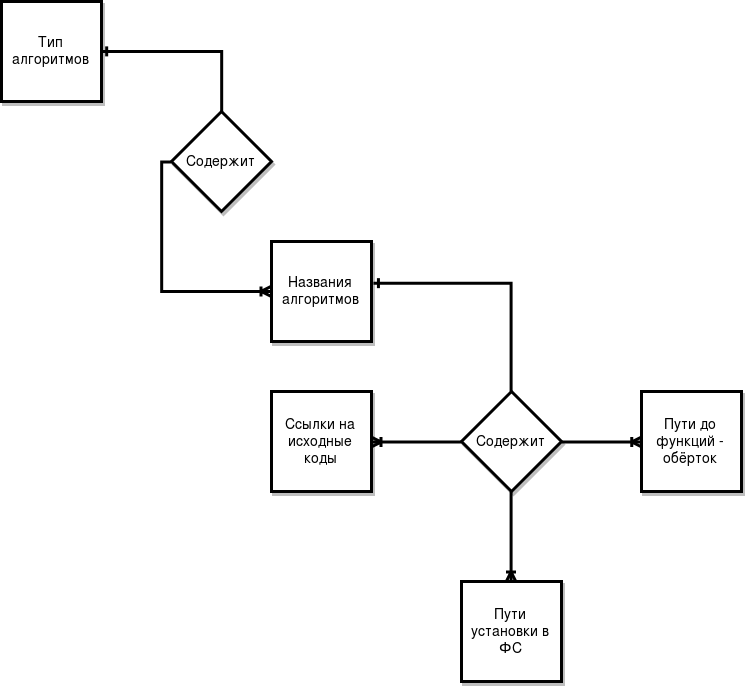
\includegraphics[width=\textwidth]{images/er}
    \caption{Диаграмма отношений сущностей в реализованном хранилище}\label{er}
\end{figure}

\newpage
Метод \textbf{get} хранилища:

\begin{center}
\begin{lstlisting}
def get(name, val, default=None):
    return getattr(_kv_, name).get(val, default)
\end{lstlisting}\label{lst:get}
Листинг \ref{lst:get}: код метода get хранилища
\end{center}

Код класса хранилища:
\begin{center}
\begin{lstlisting}
class _kv_(object):
    OPTIONS = {
            'hashing':  ['SHA-256', 'SHA-512', 'Scrypt', 'KECCAK-256',
                         'KECCAK-512', 'Ethash', 'X11', 'X17', 'myr-groestl',
                         'Lyra2rev2', 'blake2s', 'blake2b'],
#...                    
    }

    LINKS = { } # ....

    UPDATE_LINKS = { } # ....

    TOINSTALL = { } # ....

    INTERFACES = { } # ....
    \end{lstlisting}\label{lst:hran}
    Листинг \ref{lst:hran}: Представление кода реализованного key-value хранилища
\end{center}





\newpage
\section{Глава 4. Проведение эксперементов}
\subsection{Анализ времени исполнения алгоритмов в реализации блокчейнов}
Была предпринята попытка замерить время исполнения всех 24 вариаций алгоритмов на следующих операциях:

\begin{itemize}
\item Генерация пары ключей (публичный-приватный)
\item Вычисления хэш-значения
\item Электронная подпись сообщения
\item Верификация сообщения
\item Время работы Proof of Work
\item Время майна одного блока
\end{itemize}

Были замерены время исполнений участков кода готовых реализаций блокчейнв,
сгенерированных при помощи разработанного компоновщика.
Замеры проводились при помощи модуля \emph{time} в Python. Дальнейший анализ и
построение графиков происходило в среде \emph{Jupyter Notebook} с
использованием модуля \underline{matplotlib}.

Была составлена таблица с записями вида \emph{[название алгоритма; функция; битрейт;
время исполнения]} размером более 1500 записей.

\begin{figure}[h!]
    \centering
    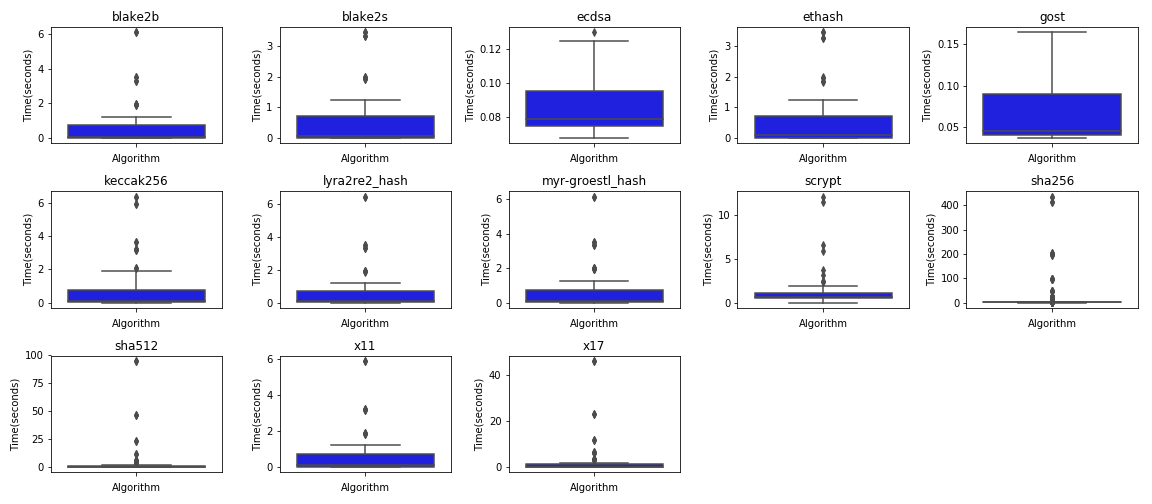
\includegraphics[width=\textwidth]{./images/boxes}
    \caption{Box-plot'ы для распределения алгоритмов по времени}\label{boxes}
\end{figure}

Далее были построены распределения общего вида (Рис. \ref{boxes}), а также
гистограммы распределения времени выполнения для алгоритмов цифровой подписи,
разделяя их на вышеперечисленные процессы (Рис. \ref{dss}):

\begin{figure}[h!]
    \centering
    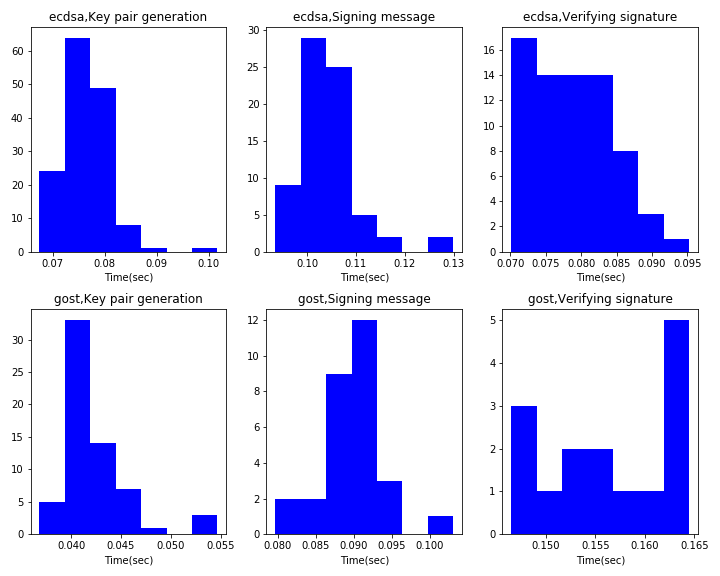
\includegraphics[width=0.68\textwidth]{./images/hists_dss}
    \caption{Распределение времени выполнения среди алгоритмов цифровой подписи}\label{dss}
\end{figure}

И аналогичные данные были построены для алгоритмов хэширования (Рис. \ref{hash}):

\begin{figure}
    \centering
    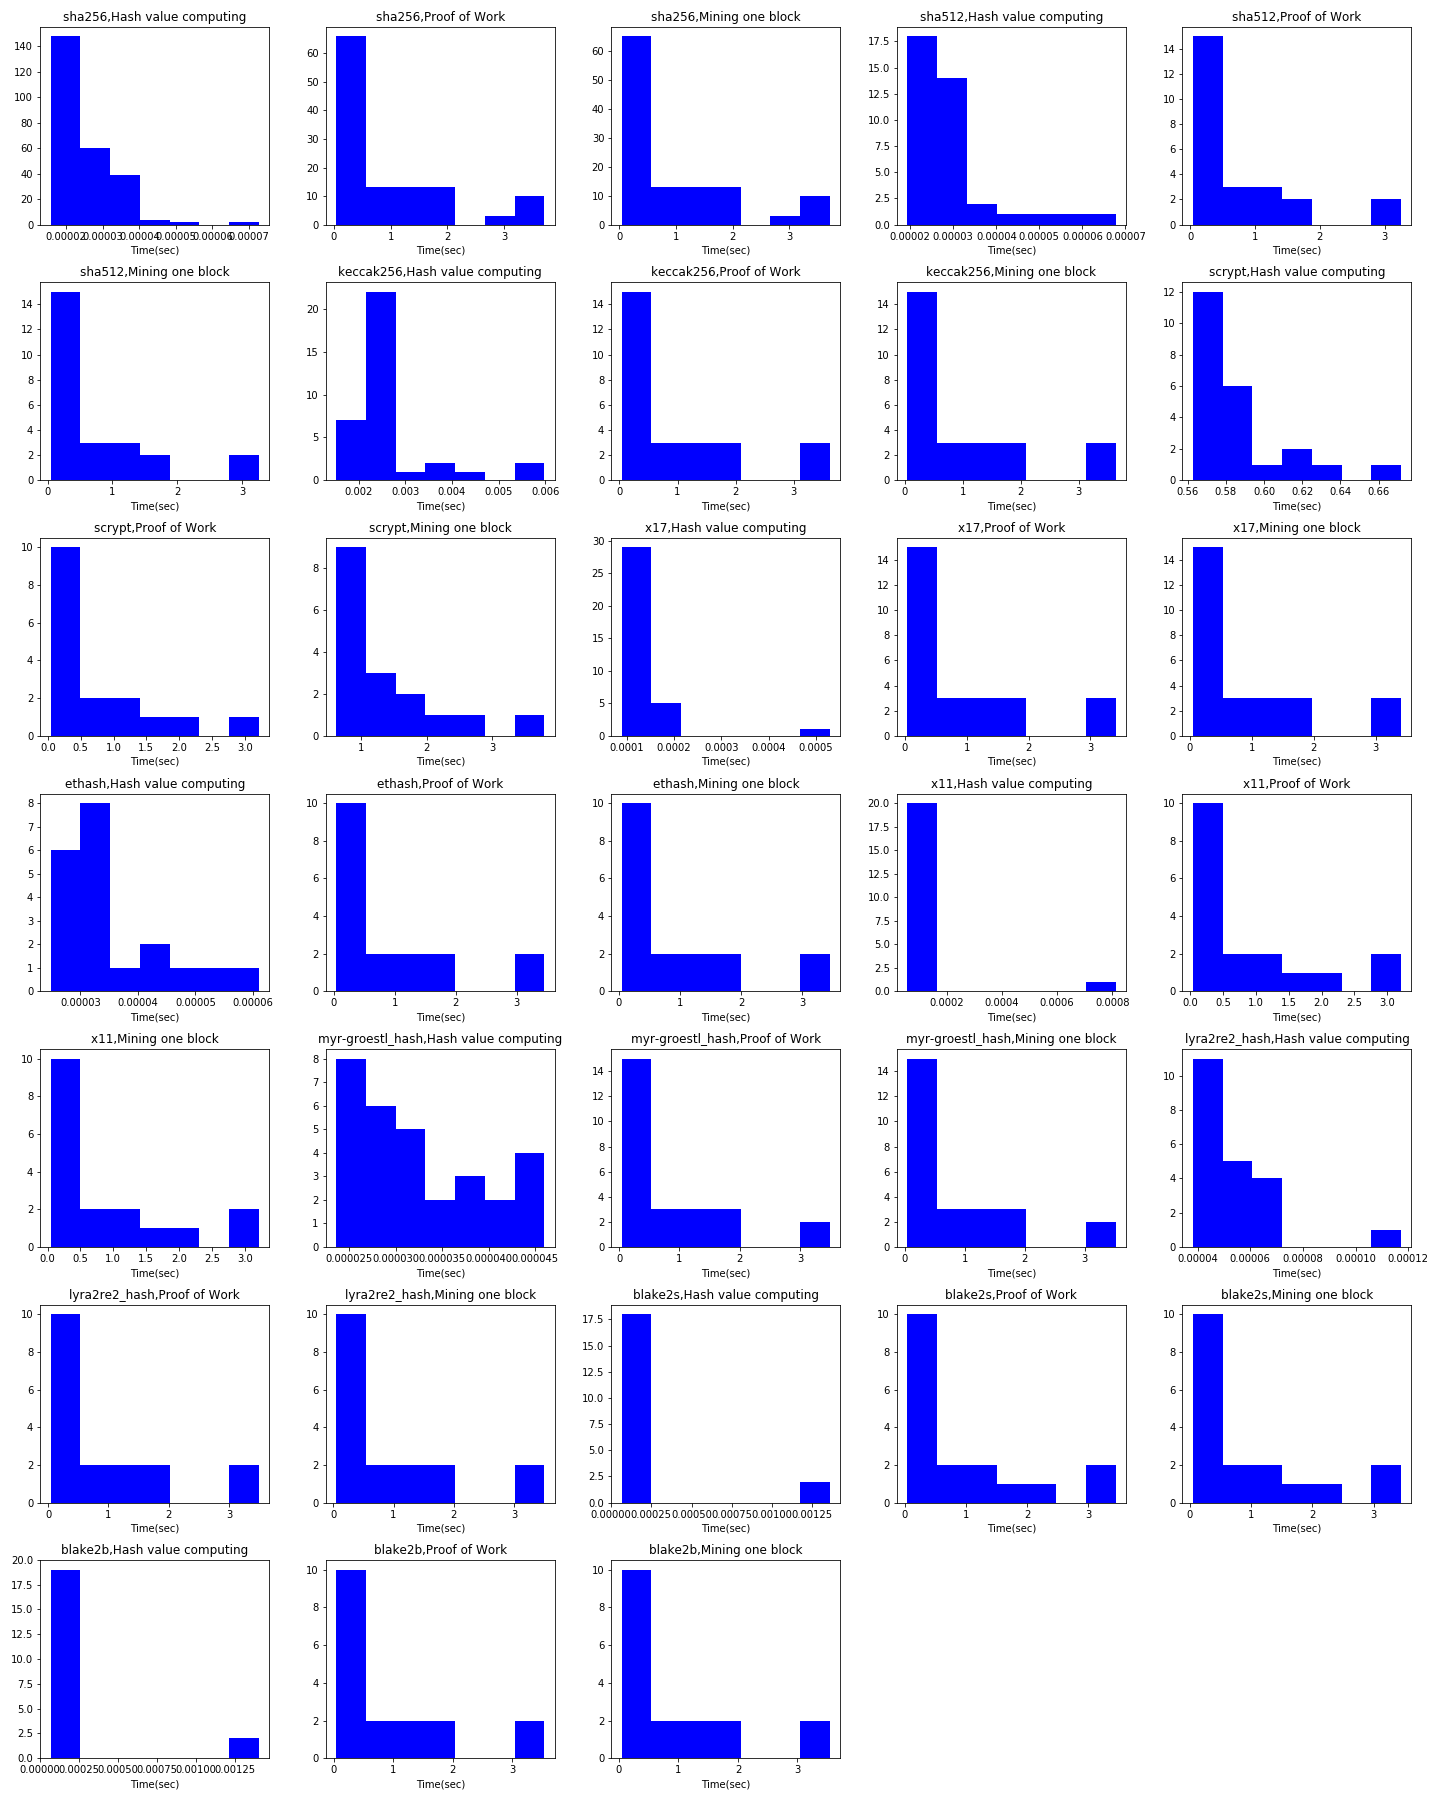
\includegraphics[width=\textwidth]{./images/hists_hashing}
    \caption{Распределение времени выполнения среди алгоритмов хэширования}\label{hash}
\end{figure}

С целью сравнить время исполнения алгоритмов по одинаковым процессам,
расположим их на одном графике гистограммы.  На Рис. \ref{boxes} с бокс-плотами
были видны выбросы, поэтому для усреднения значений на последующих графиках,
были взяты медианы значений, поскольку данные показатель более устойчив к
выбросам, чем обычное среднее.

\begin{figure}[h!]
    \centering
    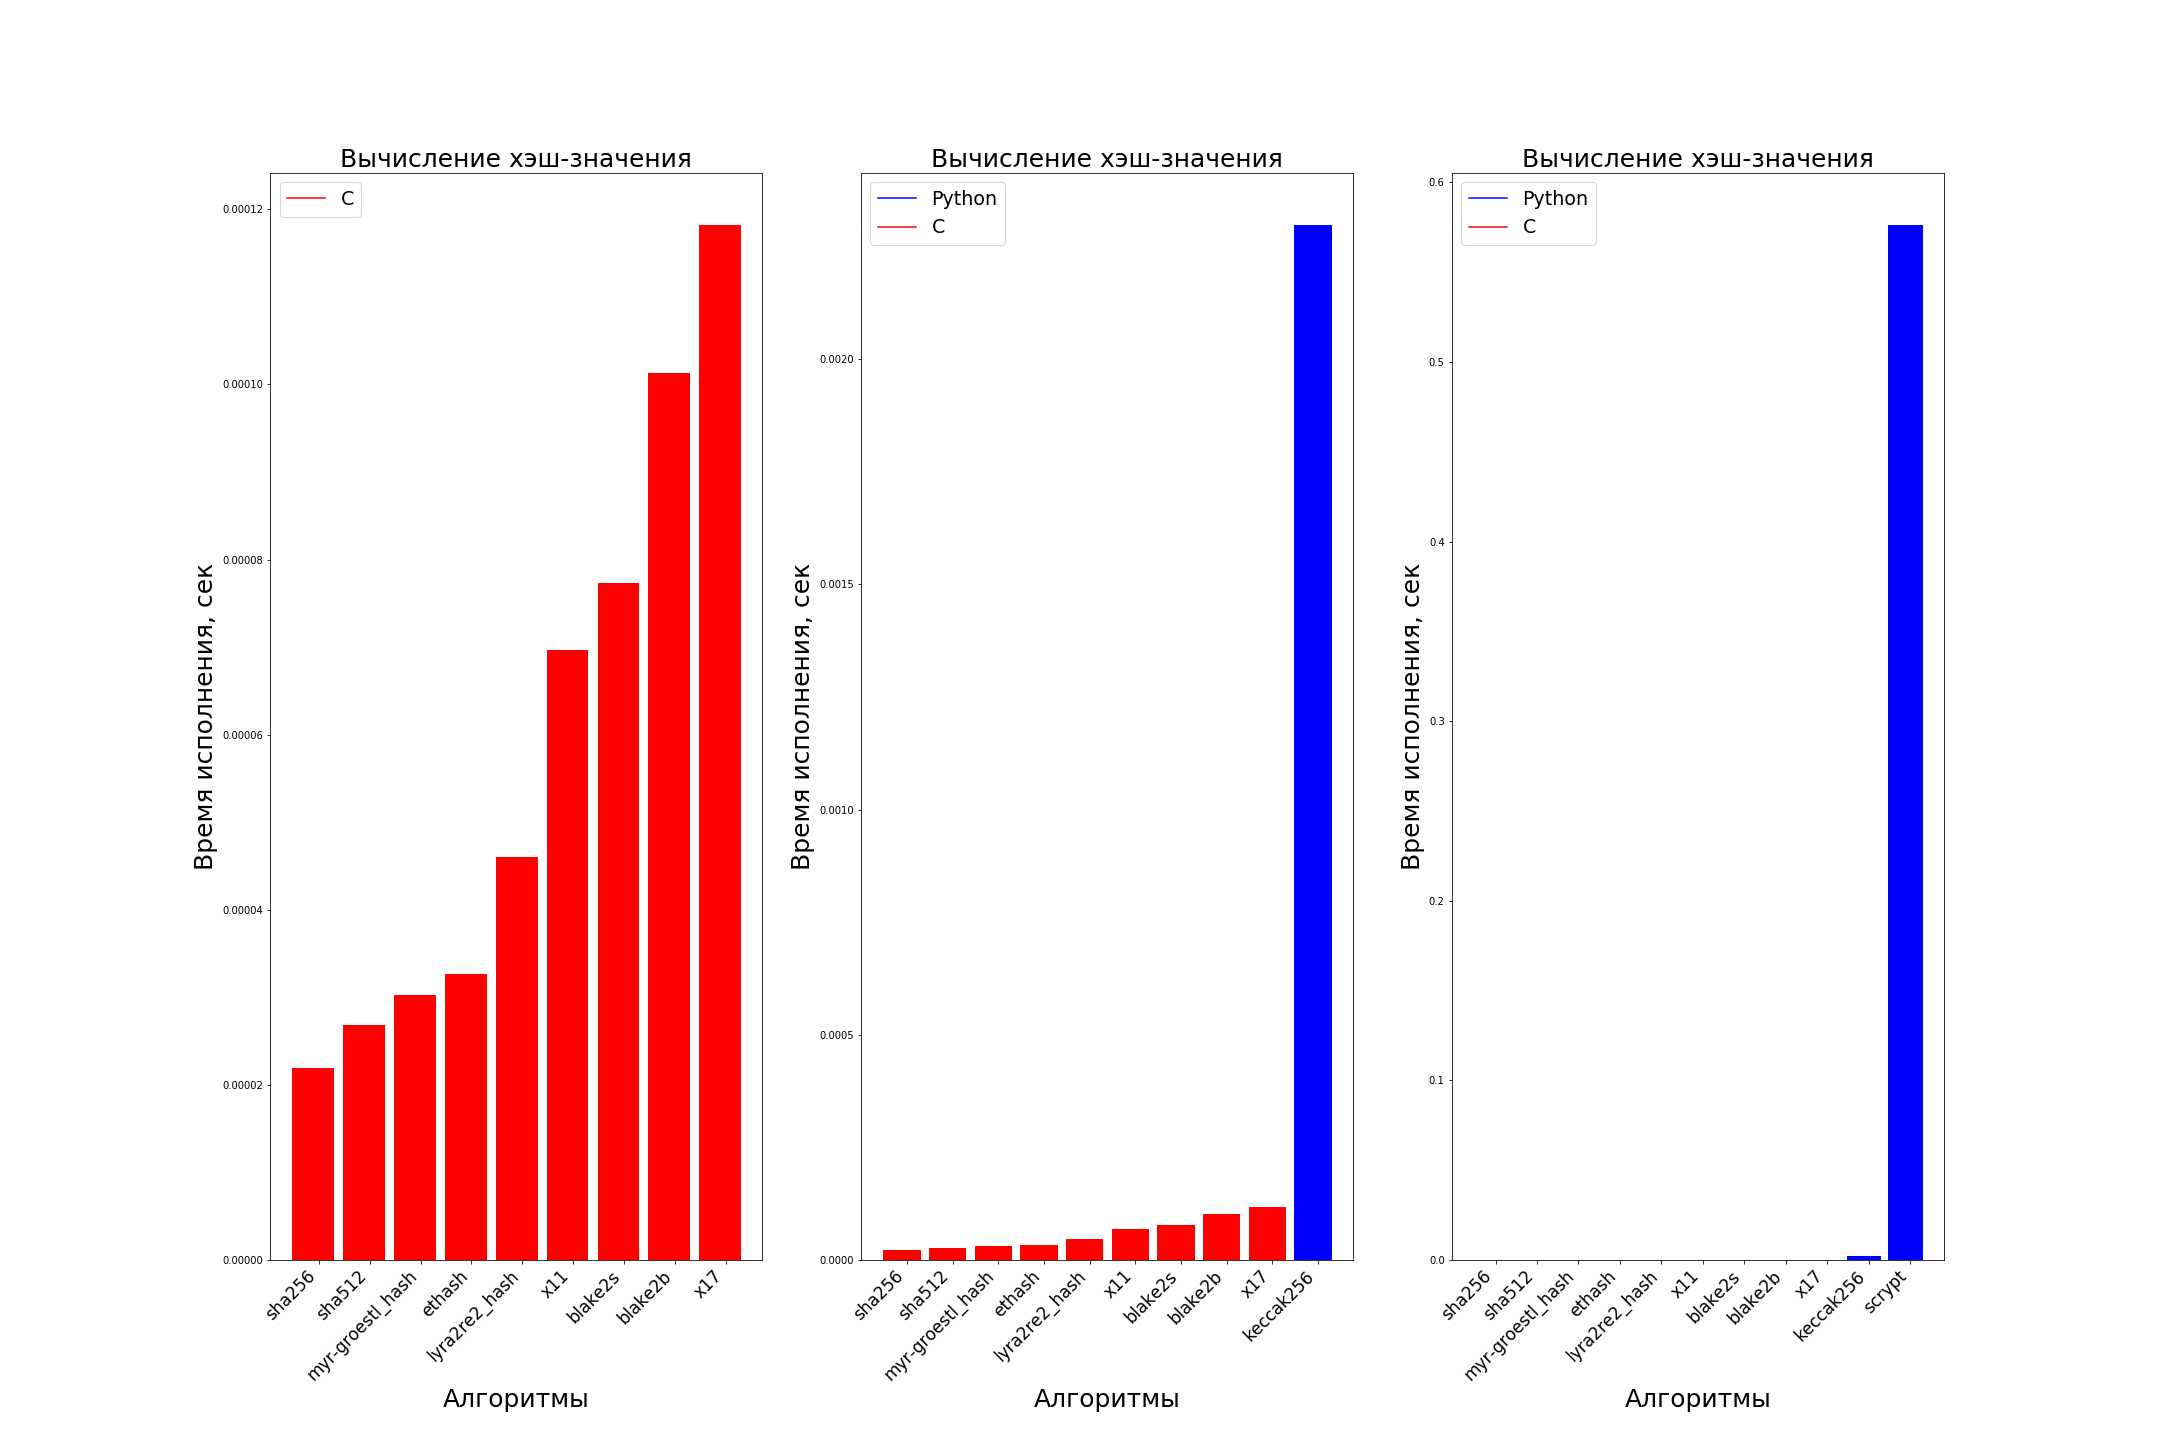
\includegraphics[width=\textwidth]{./images/hash_comparison}
    \caption{Сравнение времени исполнения работ различных алгоритмов хэширования на одинаковых функциях}\label{hash_comp}
\end{figure}

Самым быстрым алгоритмом хэширования \emph{среди упомянутых}, исходя из
проведённого анализа, является, SHA-256. Самым медленным из реализованных на
языке СИ --- X17.  На данных графиках интересно заметить, что оба алгоритма,
реализованные на языке Python, имеют гораздо большее время исполнения, по
сравнению с реализованными на языке СИ. Алгоритм ГОСТ 34.10-2012 проигрывает
международно известной ECSDA лишь во времени исполнения процедуры
верификации (Рис. \ref{dss_comp}).

\begin{figure}[h!]
    \centering
    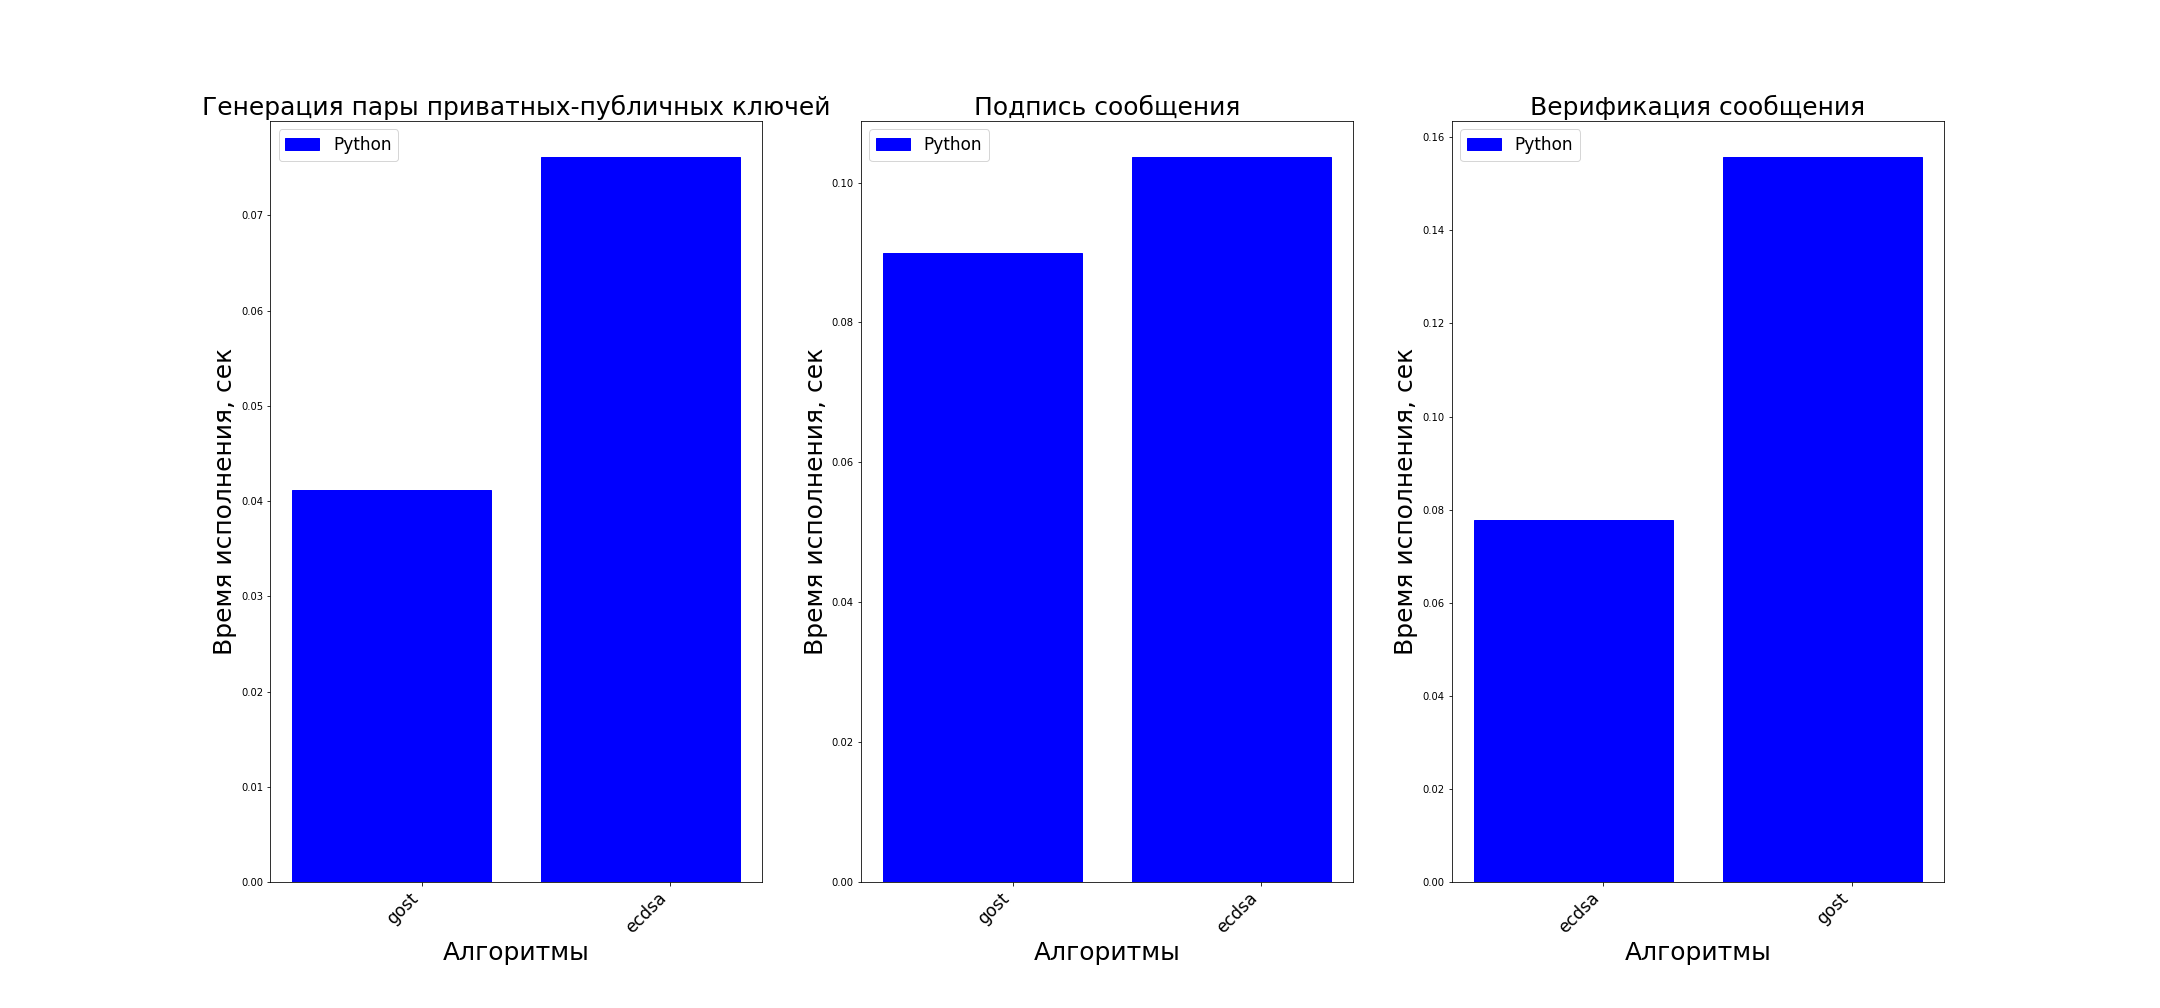
\includegraphics[width=1.\textwidth]{./images/dss_comparison}
    \caption{Сравнение времени исполнения работ различных алгоритмов цифровой подписи на одинаковых функциях}\label{dss_comp}
\end{figure}


\newpage
\subsection{Выводы}
Рассмотренные временные показатели алгоритмов могут дать пользователю
представление о том, каким будут временные показатели его блокчейна. Данное
сравнение позволит пользователю ориентироваться при выборе желаемой
конфигурации.


\newpage
\section{Заключение}
% В работе были рассмотрены использования современных алгоритмов и протоколов в
% распределенных реестрах, была актуализирована их классификация. Наличие такого
% объёма алгоритмов по защите конфиденциальности и приватности сигнализирует о
% явных проблемах в данной области. И действительно, как показало исследование,
% даже такие алгоритмы как Coinshuffle и Stealth Address не гарантируют
% анонимность отправителей и получателей. Реализация современных распределённых
% реестров предполагает гибкость и адаптируемость под новые алгоритмы и
% протоколы, которые появляются каждый месяц. В будущем мы надеемся увидеть
% прогресс в области разработки новых (основанных на свежих идеях) алоритмов и
% протоколов, что приведёт к скачку и новому всплеску популярности распределённых
% реестров в обществе.

% Написанная библиотека доступна для свободной установки и помогает разобраться в
% практических реализациях написанных алгоритмов, а так же даёт возможность
% построить учебную версию распределённого реестра. %(\ref{pril1}).


Было проведено исследование использования различных алгоритмов и протоколов в
распределённых реестрах. Были найдены новые типы распределённых реестров, такие
как Holochain, Hashgraph и Tempo. Это позволило решить проблему устаревшей
информации по классификации алгоритмов и протоколов в распределённых реестрах.\\
Была разработана актуальная классификация использования алгоритмов и протоколов
в распределённых реестров, в которой отражено современное многообразие
технологичных подходов к решению проблем безопасности.

Было разработано гибкое, масштабируемое программное средство для автоматизации
работы программирования. Разработан уникальный процесс по работе с исходными
кодами алгоритмов, расположенных удалённо, их использованию и автообновлению.
Налажена самоподдерживаемая система, не требующая вмешательства программиста
после её первичной настройки. Приложение находится в публичном доступе и
доступно к
установке.

В то же время, в работу данного приложения может быть внесён ряд
усовершенствований, возможными направлениями которых являются:
\begin{itemize}
    \item Добавление возможности генерации года не только блокчейна, но и
          других реестров
    \item Добавление в реализацию блокчейна алгоритмов по защите приватности
    \item Улучшение временных характеристик алгоритмов, реализованных на Python
          путём имплементации их на языке CИ
\end{itemize}

К основным направлениям дальнейшей работы над исследовательской частью работы
можно отнести:
\begin{itemize}
    \item Исследование работы внутренней структуры новых реестров
    \item Сравненительный анализ блокчейна и новых реестров
    \item Поддержание разработанной классификации в актуальном состоянии
\end{itemize}



\newpage
\section{Список использованных источников}
% \nocite{*}
% \printbibliography{}


% \newpage
% \section*{Приложение 1. Техническое задание}\label{tz}

\end{document}
